\documentclass[a4paper,final,headinclude=true,footinclude=true, headsepline=1pt]{scrreprt}
%bei documentclass footsepline=1pt einfügen für linie ober fußzeile

\usepackage[utf8]{inputenc}
%für die € Zeichen
\usepackage{eurosym}
%table
\usepackage{booktabs}
%Zeilenabstand
\usepackage{setspace}
\usepackage{wrapfig}
%für Rechtschreibkorrektur
\usepackage[english]{babel}
%sorting=none sortiert alles nach dem 1. Vorkommen
\usepackage[backend=biber]{biblatex}
\addbibresource{bibliography/main.bib}

%Grafiken rotieren
\usepackage{rotating}
%Subsubsections nummerieren und in Table of contents anzeigen
\setcounter{secnumdepth}{3}
\setcounter{tocdepth}{3}

%Urls in Bibliographie Zeilenbrechbar machen
\setcounter{biburlnumpenalty}{100}
\setcounter{biburlucpenalty}{100} 
\setcounter{biburllcpenalty}{100}

%fixed float@addtolists detected(scrreprt) - KOMA-Script Verbesserungen
\usepackage{scrhack}

%damit biber und glossaries zusammen funktioniert
\usepackage{csquotes}

%für code highlighting
\usepackage{minted}
%für Bilder
\usepackage{graphicx}
\usepackage{setspace}

%zeilenabstand setzen
\renewcommand{\baselinestretch}{1.3}

%headerpackage
\usepackage{scrlayer-scrpage}
\clearscrheadfoot
\pagestyle{headings}
%lo = left outer
\lohead{\headmark}
%für seitenzahl
\ofoot[\pagemark]{\pagemark}
\automark[chapter]{chapter}
\renewcommand*{\chapterpagestyle}{headings}

\newcommand{\pageauthor}[1]{\ifoot{#1}}
\newcommand{\clearpageauthor}{\newpage \ifoot{}}







\usepackage[bookmarksnumbered=true 
%Kapitel und Abschnittsnummern bei pdf Lesezeichen
]{hyperref}

\usepackage[toc]{glossaries}
\makeglossaries

%pk,shortcut,long
\newacronym{rpi2}{RPi2}{Raspberry Pi 2}
\newacronym{gps}{GPS}{Global Positioning System}
\newacronym{api}{API}{Application Programming Interface}
\newacronym{htbla}{HTBLA}{Höhere Technische Bundeslehranstalt}
\newacronym{co2}{CO2}{Carbon Dioxide}
\newacronym{ssh}{SSH}{Secure Shell}
\newacronym{rest}{REST}{Representational State Transfer}
\newacronym{mysql}{MySQL}{MY Sequential Query Language}
\newacronym{led}{LED}{Light-emitting Diode}
\newacronym{php}{PHP}{PHP Hypertext Preprocessor}
\newacronym{umts}{UMTS}{Universal Mobile Telecommunications System}
\newacronym{erd}{ERD}{Entity Relationship Diagram}
\newacronym{ddl}{DDL}{Data Definition Language}
\newacronym{dml}{DML}{Data Manipulation Language}
\newacronym{uuid}{UUID}{Universally Unique Identifier}
\newacronym{gbitps}{Gbit/s}{Gigabit per second}
\newacronym{csv}{CSV}{Comma-separated values}
\newacronym{pdf}{PDF}{Portable Document Format }
\newacronym{ios}{iOS}{iPhone Operating System}
\newacronym{html}{HTML}{Hyper Text Markup Language}
\newacronym{xml}{XML}{Extensible Markup Language}
\newacronym{pc}{PC}{Personal Computer}
\newacronym{ip}{IP}{Internet Protocol}
\newacronym{url}{URL}{Uniform Resource Locator}
\newacronym{json}{JSON}{JavaScript Object Notation}
\newacronym{db}{DB}{Database}
\newacronym{gpio}{GPIO}{General Purpose Input Output}
\newacronym{mb}{MB}{MegaByte}
\newacronym{ma}{mA}{milliampere}
\newacronym{bl}{BL}{Business Logic}
\newacronym{nan}{NaN}{Not a Number}
\newacronym{usb}{USB}{Universal Serial Bus}
\newacronym{ups}{UPS}{Uninterruptible Power Supply}
\newacronym{tvnc}{TightVNC}{Tight Virtual Network Computing}
\newacronym{uart}{UART}{Universal Asynchronous Receiver Transmitter}
\newacronym{gpsd}{GPSD}{GPS Daemon}
\newacronym{gpx}{GPX}{GPS Exchange Format}
\newacronym{wlan}{WLAN}{Wireless Local Area Network}
\newacronym{lan}{LAN}{Local Area Network}
\newacronym{kml}{KML}{Keyhole Markup Language}
\newacronym{nmea}{NMEA}{National Marine Electronics Association}
\newacronym{os}{OS}{Operating System}
\newacronym{ide}{IDE}{Integrated Development Environment}

\begin{document}
\titlehead{\begin{minipage}[hbt]{5cm}
\centering

\includegraphics[width=5cm]{bilder/htblaKaindorf.pdf}
\end{minipage}
\hfill
\begin{minipage}[hbt]{5cm}
\centering
\vspace{25px}

\includegraphics[width=5cm]{bilder/informatikLogo}
\end{minipage}}
\title{driver's logbook}
\author{Helena Adam, Claudio Knapp, Laura Rössl, Paul Zwölfer}
\date{\today}

\maketitle
\chapter*{Abstract}
\addcontentsline{toc}{chapter}{Abstract}
Every day people go to work with their own or the company's car. To get taxes from the company for their driven kilometers, they always have to note down how many kilometers they drove for private and business purposes, which is a lot of work. But nevertheless it has to be done, because it gets added to the income. The private use of vehicles gets scheduled with 2\% of the acquisition cost. At vehicles with a lower CO2 emission value the schedule is 1.5\% of the acquisition cost.
\newline \newline
Our Project consists of a device which is placed in a car. This hardware consists of an \gls{rpi2} and a \gls{gps} module. It tracks the distance and sum up the kilometers, which are driven by the car driver. This information gets inserted into a database. If there is no internet connection at the moment, the data is saved on the device and uploaded as soon as possible if there is an internet connection available. Afterwards, the user can log into his user account on our website or mobile application to see the tracks he or she drove. The user also can enter routes manual with the app or on the website. This can be separated in private and business usage of the car from the user. The possibility to edit the tracked ways is also given. Its also possible to view it on the phone or tablet via an mobile application.
\newline \newline
To sum up, we provide a device with a software on it, to create tracks via \gls{gps} data while driving. These are saved online and can be viewed on a website or mobile application.
\chapter*{Acknowledgements}
\pageauthor{Helena Adam}
We want to thank a lot of people. On the one hand, those people, who even made it possible for us to attend the \gls{htbla} Kaindorf. On the other hand, those who contributed valuable help to create a successful diploma-thesis.

A thank goes to all employees of our diploma-thesis company, Sunlime IT Services GmbH, who supported us in our work. However, a special thanks goes to our employer DI Dominik Fuchshofer, who gave us the chance to do our diploma-thesis with his company. As contact person he always stood at our side whenever we needed assistance. Without his tireless input, patience and understanding our problems it would not have been possible to successfully complete the diploma-thesis.

Furthermore, we would like to thank DI Dr. Wolfgang Pölzleitner and DI Florian Schreiber, who took over the role as our supervisor teachers. When we had problems or other blockades, they always were there to help us finding a solution and make the best out of it. Through their cheerful character and their great interest in our work, we had good times at our meetings with them together.

Then, we want to thank our head teacher Mrs. Mag. Michaela Primig, who supported us the last past years. Sometimes we were not that easy, but she never lost hope that we could not manage anything we wanted to do.

Last but not least, our deep thankfulness needs to be expressed to our parents. They supported us during our \gls{htbla} career and gave us motivation whenever we needed one. Anyway, a special thanks goes to Pauls dad, who helped us a lot with our diploma-thesis.
\clearpageauthor


\chapter*{Project Members}
\section*{Helena Adam}
Helena took over the task of the team leader of this project. She was our connection person to our supervising teachers and our partner company. She managed the task of comparing competitive products and documented held meetings.
\begin{center}
%\includegraphics[width=0.85\textwidth]{Helena}
\end{center}
\section*{Claudio Knapp}
Our hardware expert Claudio cared about our hardware prototype and additional modules we appended. ...
\begin{center}
%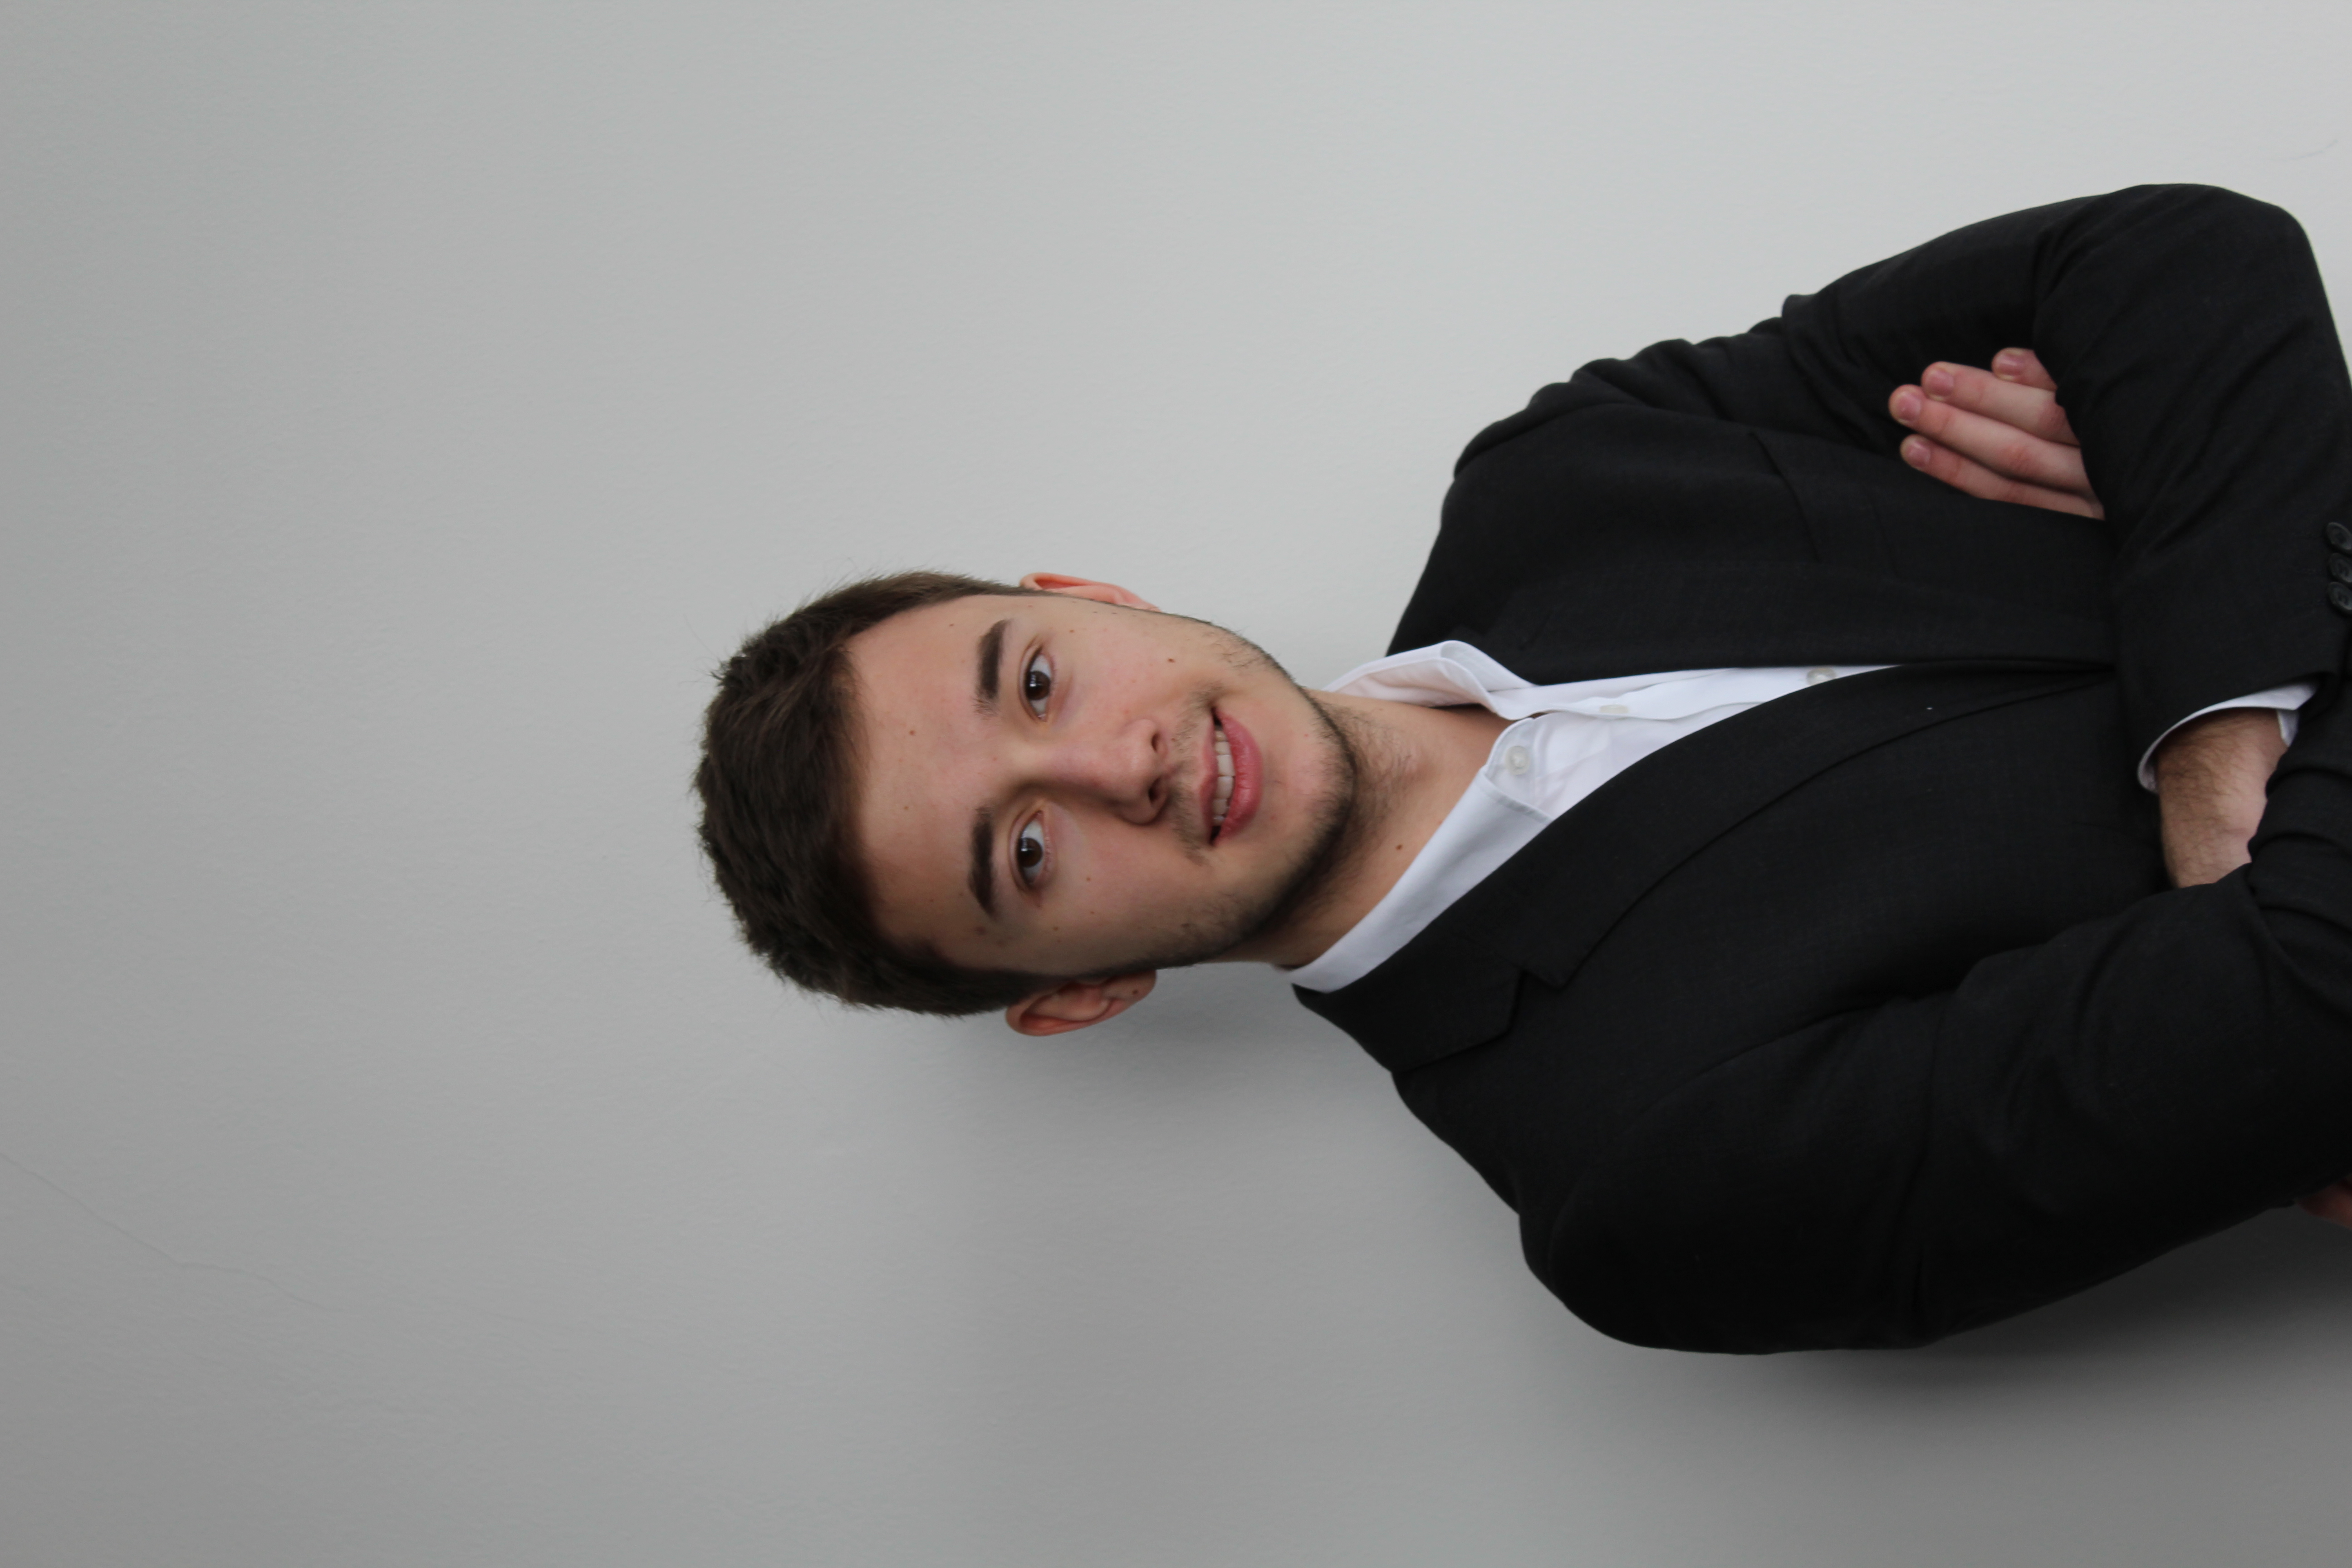
\includegraphics[width=0.85\textwidth]{Claudio}
\end{center}
\section*{Laura Rössl}
The role of the \gls{db} expert was taken over by Laura who set up and maintained our \gls{db}. ...
\begin{center}
%\includegraphics[width=0.85\textwidth]{Laura}
\end{center}
\section*{Paul Zwölfer}
The main task of Paul was to set up and update our software. ...
\begin{center}
%\includegraphics[width=0.85\textwidth]{Paul}
\end{center}
\chapter*{Statutory Declaration}
\addcontentsline{toc}{chapter}{Statutory Declaration}
With this I declare that all work presented in this diploma thesis is my own mindwork. I have used only the referred sources and aids and all parts which have been either literally or in general manner from other sources have been indicated accordingly.
\newline \newline
Furthermore, the secondary technical school HTBLA Kaindorf/Sulm is privileged to use any of my work included in this diploma thesis for educational or research purposes, as long as special attention is paid to data security and competitional regulations.
\tableofcontents
\chapter*{Foreword from the Employer}
Kilometre allowance and the documentation of driven kilometres for the company are important todos for every self employed entrepreneur. The fact is that writing every business car ride into an excel sheet or manually into a car log book is really annoying. It would be much more convenient if a device in my business car logs every trip and I am able to define my car rides via a web portal afterwards. This was the idea behind “Log book” which we wanted to test drive with our friends at HTBLA Kaindorf/Sulm. Next to the hardware prototype it was also important to get an idea for a possible database solution. To understand the project better we provided a design proposal next to the hardware to sum up the first section of the project.

But more important than the final outcome of the project is to see how young people are able to come up with new and interesting ideas and dive into project related subtasks which have to be accomplished. It is also great to transfer some of the know-how we have worked out and to see how these ideas are adopted and developed for the project.

I am sure that every project member is able to take something from this diploma thesis and use it for their own future business life. I wish Helena, Laura, Claudio and Paul the very best for the final exams. You are going to rock the stage.

  Best,\newline
Dominik\newline\newline
DI Dominik Fuchshofer, BSc\newline
CEO/CTO at Sunlime IT Services GmbH\newline
February 2016

\markboth{Introduction}{Introduction}  
\chapter*{Introduction}
\addcontentsline{toc}{chapter}{Introduction}
\section*{State of the Art}
Until now, the company has to track the driven distance by hand. They note down different parameters in an EXCEL sheet. There is a separate sheet for each month of the year. These parameters include the date, tachometer kilometers at the beginning and the end of the trip, how much kilometers are driven for the company or private use, the route they took, and the reason for driving.

This method is very time consuming and has to be done for every company related trip. Non company related trips must be excluded.
\subsection*{Our functionalities}
The \gls{rpi2} powers up when the driver starts up the car's ignition. After that, the autostart routine starts our software, including the process of collecting \gls{gps} data, saving and uploading it.

When the software started up, it checks if there is some \gls{gps} data from previous tracks to be uploaded. If that is the case, this data will be read from the save.jPoint file into the queue. After that, the save thread uploads a maximum of 50 points to the \gls{rest} service. 


Then the \gls{gps} data of the current track gets saved via the API thread into the queue and then synchronized with the save.jPoint file.

Reading and writing data simultaneously is possible due to the use of a blocking queue. This type of list manages the access of the list so that no errors occur.\newline
Successfully uploaded points are removed from the list and therefore from the synchronized backup file.

This runs through as long as the \gls{rpi2} is supplied with power.


\newpage
\section*{Role of the Company}
In this part of our diploma-thesis it is listed up what our employer, Sunlime IT Services, contributes to the work of the electronic logbook. Following areas are included:
\begin{itemize}
\item Hardware
\item Data transfer
\item Design requirements
\item Content requirements
\end{itemize}
The company provides the \gls{rpi2} with all the components like \gls{gps} Module or antenna to create a working hardware prototype for the logbook.

Secondly, at the data transfer, they will define when and over which portal the data has to be sent. Moreover, it should be apparent which user is transferring the data, so it can be dedicated online. It is also important to consider the user data when designing the \gls{db}. Furthermore, a feature list has to be defined and integrated.
The web server for the portal is also provided and maintained from the company.

An external service provider creates the design from the existing wireframing and Sunlime IT Services implements the technical aspects to it. The external service provider should also design a Logo for the product.

Thirdly, the company has to choose a “Mobile-first” approach to react to the display measures of each end device.

Then, the logbook should also work on smartphones. Therefore, Adobe PhoneGap will help to transact the program. The mobile application has to be designed one time only.

Finally, the company is responsible for the security on the servers. It should not be possible to have access on a server as third person. Passwords are only allowed to get saved encrypted.
\newpage
\section*{Goals}
The goal of our diploma-thesis is to build a working hardware prototype. This is recording the driven \gls{gps} data. A \gls{rpi2} with a \gls{gps} module has to be placed in a car. The prototype tracks \gls{gps} data and transfers it to the \gls{rest} service. \gls{rest} is responsible for uploading data into the \gls{db}. 

In case there is no internet connection, we store the \gls{gps} data locally. The program structure is described in our Software description section.

Information about the user and the tracks have to be stored in the \gls{db}. We also created and designed a \gls{erd} to illustrate the structure of the \gls{db}. Furthermore, the \gls{ddl} and the \gls{dml} resulted out of the \gls{erd}.

The wireframing is the Front-End representation of our diploma thesis. It displays the user interface on our web portal and mobile application. The result of it is a user-friendly design.

To get a unique product, the market needs to get analysed. Here, the competitors should get detected and compared in different attributes. For instance: costs, supported platforms, \gls{gps}, hardware etc. With this information, we create a diploma-thesis that differs from other products. Furthermore, other intended uses of the hardware prototype should get noted down.

Last but not least, the project management of the working packets has to be defined appropriate and documented.

\chapter{Project Management}
\section{Scrum}
\subsection{Description of Scrum}
Scrum is an iterative and incremental agile process used to develop software. The team had to self-organize itself by taking the tasks from the scrum board.

At the beginning of developing the product, the project goals got divided into sprints by the team. To have an overview over the whole project, the so called scrum meetings were held. During these scrum meetings, the points that have already been done and what’s still left in this sprint, got discussed. Those discussions can be held daily by the project team and should help to see the process in the project in a certain time.

Three different roles are represented in Scrum. Firstly, the development team. They are responsible for the programming part of the software. Secondly, the product owner. He provides the user stories the development  team has to do. Moreover, to keep the customer satisfied, he makes sure that the software has included everything the customer requested. Last but not least, the Scrum master. Disturbances can delay the milestones deadlines. To prohibit this, he makes sure that the development team can work efficient without the project managers or the customers interference.
\subsection{Why we have chosen Scrum}
As already mentioned above, scrum is agile because of the sprints. Basically, it means that there is no problem in changing or adding sprints in the current tasks without a delay. We have already had a good experience with Scrum in the 3rd grade. So, we already knew that Scrum works really good with managing changes. As it was our first “big” project and we had no idea how often we could change our project, we decided on Scrum.

\section{Project Organization Chart}
The following diagram shows the structure of the organization. It pictures who was involved, what their position in the project was and their relation to each other. 

Our contact person for our diploma-thesis was DI Dominik Fuchshofer. He is the \gls{ceo} of the company Sunlime IT Services, we created our work for. Our two supervisors DI Dr. Wolfgang Pölzleitner and DI Florian Schreiber took care of the progress we made. The members of our project team are Helena Adam, Claudio Knapp, Laura Rössl and Paul Zwölfer. Everyone communicated with the employer on its own, over Hangouts.
\begin{center}
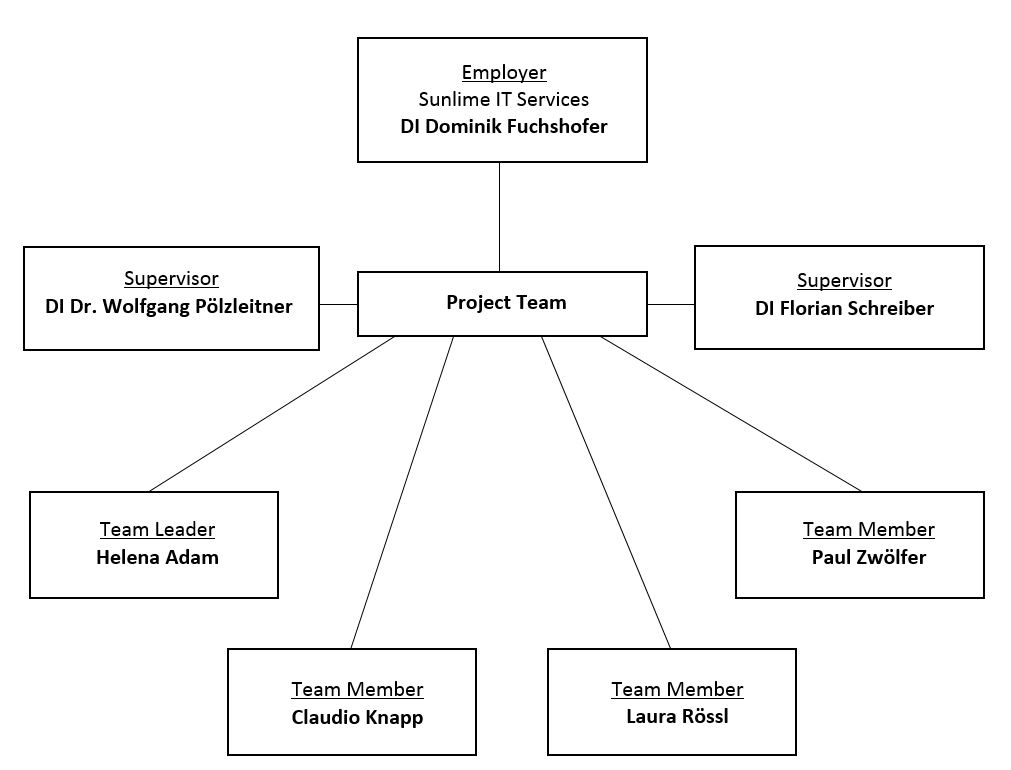
\includegraphics[width=0.8\textwidth] {bilder/projectdiagram}
\end{center}
\newpage
\section{Milestones}
Milestones are tools for the project management to schedule the project. The present work gets divided into some parts. Then, it gets defined until when a part has to be done. This tool is used to avoid bigger delays in this project.\newline

In the chart below it is visible into which parts we have divided out diploma-thesis and the date until it was due.\newline
\begin{center}
\begin{tabular}{p{5cm}p{5cm}}
\toprule
Competitor analysis & July 10, 2015 \\
Wireframing & July 31, 2015 \\
Designing of data & November 24, 2015 \\
Functioning software & January 12, 2016 \\
Hardware prototype & February 16, 2016 \\
Bug fixing & February 23, 2016 \\
Documentation & \today \\
\bottomrule
\end{tabular}
\end{center}
\section{Working Hours}
Here you can see a listing of our working hours and how much time we spent on different tasks. You can see in the following table that we spent the most hours on documentation of the diploma thesis. The main reason for this is the technology LaTeX we used. \newline
\begin{center}
\begin{tabular}{p{5cm}p{2cm}}
\toprule
\textbf{Type} & \textbf{Hours} \\
\midrule
Administration & 194,05 \\
Designing & 7 \\
Data design & 43 \\
Documentation & 225,7 \\
Programming & 179,75 \\
Research & 85 \\
Raspberry Pi & 140 \\
Testing & 18 \\
UML Diagrams & 14 \\
Wireframing & 81 \\
\bottomrule
\end{tabular}
\end{center}
\chapter{Software Requirements}
\section{Intially}
\subsection{Data Transmission}
It has to be clear when a transmission takes place and which data it contains. The user who is getting tracked must be recorded for the \gls{db} too.
\subsection{Data Design}
Also the information about the users have to be stored in the \gls{db}. Furthermore, a list of features has to be defined and integrated. This serves to adapting extensions of products from the competitive analysis.
\subsection{Webserver}
The webserver is provided and maintained by the company Sunlime IT Services. The server is located in a data center in Vienna and is tethered with 10\gls{gbitps}.
\section{Additional Requirements}
\subsection{REST}
We switched to the technology \gls{rest} to save data in the \gls{db}. Our \gls{rest} Server is written in \gls{php} and uploads data.
\subsection{MySQL Database}
Since our partner companies main products are homepages, they already had a running \gls{mysql} \gls{db}. So they created a new workspace for us, which we could use.
\chapter{Competitor Analysis}
\pageauthor{Helena Adam}
\section{Introduction}
In this part of our diploma thesis we give you some information about our current competitors we are sharing our project idea with.

One important factor to create an outstanding product and to lead the market is to know our competitors. Like it is said “Keep your friends close, but your enemies closer”. So we were supposed to do some researches about similar products. They are listed on the next few pages. We try to sum up the most important facts and a short description of the products competing. 

The competitor analysis showed us what we have to look at and what customers exactly need. \newline \newline
\begin{singlespace}
\textbf{Compared Products}
\begin{itemize}
\item Miles
\item OsmAnd
\item TOMTOM
\item Fahrtenbuch (von Stefan Meyer)
\item TOUR
\item Mileage Logbook
\item Fahrtenbuch (myLogbook)
\item MyLog GPS Fahrtenbuch Kosten
\item Carpanion
\item Fahrtenbuch Mileage Book
\item Trucker Logbook
\item Logbuch App
\item Drives Fahrtenbuch
\item Abax Triplog
\item GPS Log Book
\item GPS Log Book Live
\item Gurtam
\item Maxtech
\item Tractive
\end{itemize}
\newpage
\clearpageauthor
\section{Miles}
\pageauthor{Claudio Knapp}
\begin{wrapfigure}{r}{0.5\textwidth}
  \begin{center}
    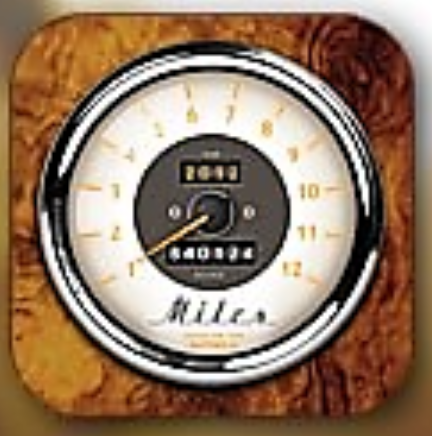
\includegraphics[width=0.48\textwidth] {bilder/miles}
  \end{center}
\end{wrapfigure}
\textbf{Costs} \euro 39,99 once\newline\newline
\textbf{Supported Platforms} The application Miles is compatible for \gls{ios} 8.\newline\newline
\textbf{GPS} No \gls{gps} connection necessary.\newline\newline
\textbf{Business/Private mode} You can split your private tracking from your business tracking.\newline\newline
\textbf{Hardware} No Hardware. App is only used on smartphones.\newline\newline
\textbf{Access Forms} App\newline\newline
\textbf{Manual/Automatic Tracking} Data can only be entered manually.\newline\newline
\textbf{Internet Connection} Internet connection necessary.\newline\newline
\textbf{Export} It’s possible to export data to a \gls{pdf} or \gls{csv} File.\newline\newline
\textbf{Other Features} No other features included.\newline\newline
\textbf{References:} \cite{miles}
\newpage
\clearpageauthor
\section{OsmAnd} 
\pageauthor{Paul Zwölfer}
\begin{wrapfigure}{R}{0.5\textwidth}
\centering

\includegraphics[width=0.48\textwidth]{bilder/osmand.png}
\end{wrapfigure}



\textbf{Costs} \euro 6,99 once\newline\newline
\textbf{Supported Platforms} For Android and \gls{ios} smartphones and tablets. Also runs on a wide array of Linux-based systems.\newline\newline
\textbf{GPS} Navigation- and tracking  system in one.\newline\newline
\textbf{Business/Private mode} Only private mode.\newline\newline
\textbf{Hardware} No Hardware. App is only used on smartphones.\newline\newline
\textbf{Access Forms} App\newline\newline
\textbf{Manual/Automatic Tracking} automatic\newline\newline
\textbf{Internet Connection} No Internet connection necessary.\newline\newline
\textbf{Export} It’s possible to export data to a \gls{pdf} or \gls{csv} File.\newline\newline
\textbf{Other Features} download offline Maps for tracking and navigation\newline\newline
\textbf{References:} \cite{osmand}
\newpage
\clearpageauthor
\section{TOMTOM}
\pageauthor{Helena Adam}
\begin{wrapfigure}{r}{0.5\textwidth}
  \begin{center}
    
\includegraphics[width=0.48\textwidth]{bilder/tomtom}
  \end{center}
\end{wrapfigure}
\textbf{Costs} \euro 69.41 once\newline\newline
\textbf{Supported Platforms} For Android (2.3.3 or higher) and \gls{ios} (5.0 or higher).\newline\newline
\textbf{GPS} \gls{gps} connection is necessary.\newline\newline
\textbf{Business/Private mode} You can split your private tracking from your business tracking.\newline\newline
\textbf{Hardware} No Hardware. App is only used on smartphones.\newline\newline
\textbf{Access Forms} App\newline\newline
\textbf{Manual/Automatic Tracking} No information\newline\newline
\textbf{Internet Connection}No information
\textbf{Export} It’s possible to export data to a \gls{pdf} or \gls{csv} File.\newline\newline
\textbf{Other Features} No other features included.\newline\newline
\textbf{References:} \cite{Electronic_Logbook_from_TOMTOM}\newline\newline
\newpage
\clearpageauthor
\section{Fahrtenbuch (von Stefan Meyer)}
\pageauthor{Laura Rössl}
\begin{wrapfigure}{r}{0.5\textwidth}
  \begin{center}
    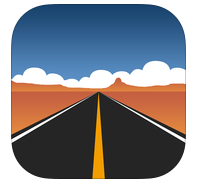
\includegraphics[width=0.48\textwidth]{bilder/fahrtenbuch}
  \end{center}
\end{wrapfigure}
\textbf{Costs} \euro 5,99 once
\newline\newline
\textbf{Supported Platforms} \gls{ios}
\paragraph{GPS} \gls{gps} connection is necessary.
\newline\newline
\textbf{Business/Private mode} You can split your private tracking from your business tracking.
\newline\newline
\textbf{Hardware} No Hardware. App is only used on smartphones.
\newline\newline
\textbf{Access Forms} App for iPhone and Apple Watch
\newline\newline
\textbf{Manual/Automatic Tracking} manual and automatic
\newline\newline
\textbf{Internet Connection} Internet connection is necessary.
\newline\newline
\textbf{Export} It’s possible to export data to a \gls{pdf} or \gls{csv} File.
\newline\newline
\textbf{Other Features} No other features included.
\newline\newline
\textbf{References:} \cite{Fahrtenbuch_von_Stefan_Meyer}
\newpage
\clearpageauthor
\section{TOUR}
\pageauthor{Claudio Knapp}
\begin{wrapfigure}{r}{0.5\textwidth}
  \begin{center}
    
\includegraphics[width=0.48\textwidth]{bilder/tour}
  \end{center}
\end{wrapfigure}
\textbf{Costs} Cost free. with features \euro 8,99 + \euro 5 to transfer the data to the computer
\newline\newline
\textbf{Supported Platforms} \gls{ios}
\newline\newline
\textbf{GPS} \gls{gps} connection is necessary.
\newline\newline
\textbf{Business/Private mode} You can split your private tracking from your business tracking.
\newline\newline
\textbf{Hardware} No Hardware. App is only used on smartphones.
\newline\newline
\textbf{Access Forms} App
\newline\newline
\textbf{Manual/Automatic Tracking} automatic
\newline\newline
\textbf{Internet Connection} Internet connection is necessary.
\newline\newline
\textbf{Export} It’s possible to export a Tax Office conform file.
\newline\newline
\textbf{Other Features}Trips can be combined afterwards
\newline\newline
\textbf{References:} \cite{TOUR}
\newpage
\clearpageauthor
\section{Mileage Logbook}
\pageauthor{Paul Zwölfer}
\begin{wrapfigure}{r}{0.5\textwidth}
  \begin{center}
    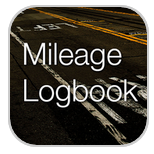
\includegraphics[width=0.48\textwidth]{bilder/mileage}
  \end{center}
\end{wrapfigure}
\textbf{Costs} free
\newline\newline
\textbf{Supported Platforms} Android 
\newline\newline
\textbf{GPS} \gls{gps} connection is necessary.
\newline\newline
\textbf{Business/Private mode} You can split your private tracking from your business tracking.
\newline\newline
\textbf{Hardware} No Hardware. App is only used on smartphones.
\newline\newline
\textbf{Access Forms} App
\newline\newline
\textbf{Manual/Automatic Tracking} automatic
\newline\newline
\textbf{Internet Connection} No internet connection is necessary.
\newline\newline
\textbf{Export} It’s possible to export data to a \gls{html}, Excel or \gls{csv} File.
\newline\newline
\textbf{Other Features} No other features included.
\newline\newline
\textbf{References:} \cite{Mileage_Logbook}
\newpage
\clearpageauthor
\section{Fahrtenbuch (myLogbook)}
\pageauthor{Helena Adam}
\begin{wrapfigure}{r}{0.5\textwidth}
  \begin{center}
    
\includegraphics[width=0.48\textwidth]{bilder/fahrtenbuch2}
  \end{center}
\end{wrapfigure}
\textbf{Costs} \euro 4,98 once
\newline\newline
\textbf{Supported Platforms} Android 
\newline\newline
\textbf{GPS} GPS connection is necessary.
\newline\newline
\textbf{Business/Private mode} Only business mode.
\newline\newline
\textbf{Hardware} No Hardware. App is only used on smartphones.
\newline\newline
\textbf{Access Forms} App
\newline\newline
\textbf{Manual/Automatic Tracking} automatic
\newline\newline
\textbf{Internet Connection} No internet connection is necessary.
\newline\newline
\textbf{Export} It’s possible to export data to a \gls{html}, \gls{xml}, INtex, Euro-Fahrtenbuch, Fahrtenbuch Express, WISO Fahrtenbuch or \gls{csv} File.
\newline\newline
\textbf{Other Features} No other features included.
\newline\newline
\textbf{References:} \cite{Fahrtenbuch_myLogbook}
\newpage
\clearpageauthor
\section{MyLog GPS Fahrtenbuch Kosten}
\pageauthor{Claudio Knapp}
\begin{wrapfigure}{r}{0.5\textwidth}
  \begin{center}
    
\includegraphics[width=0.48\textwidth]{bilder/mylog}
  \end{center}
\end{wrapfigure}
\textbf{Costs} free
\newline\newline
\textbf{Supported Platforms} Android
\newline\newline
\textbf{GPS} \gls{gps} connection is necessary.
\newline\newline
\textbf{Business/Private mode} You can split your private tracking from your business tracking.
\newline\newline
\textbf{Hardware} No Hardware. App is only used on smartphones.
\newline\newline
\textbf{Access Forms} App
\newline\newline
\textbf{Manual/Automatic Tracking} automatic
\newline\newline
\textbf{Internet Connection} No internet connection is necessary.
\newline\newline
\textbf{Export} It’s possible to export data to a \gls{pdf} File.
\newline\newline
\textbf{Other Features} No other features included.
\newline\newline
\textbf{References:} \cite{MyLog_GPS_Fahrtenbuch_Costs}
\newpage
\clearpageauthor
\section{Carpanion}
\pageauthor{Claudio Knapp}
\begin{wrapfigure}{r}{0.5\textwidth}
  \begin{center}
    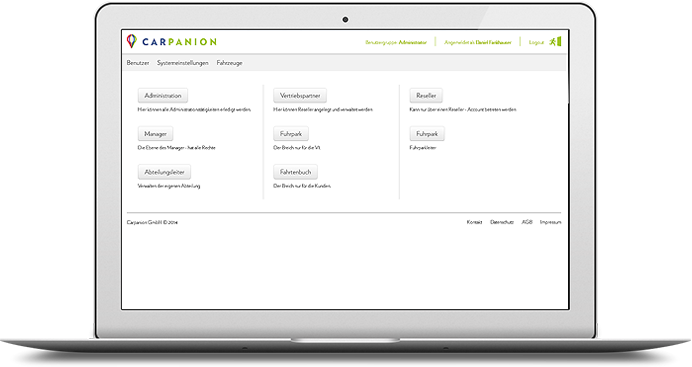
\includegraphics[width=0.48\textwidth]{bilder/Carpanion1}
  \end{center}
\end{wrapfigure}
\textbf{Costs} free
\newline\newline
\textbf{Supported Platforms} Android, \gls{ios}, Windows
\newline\newline
\textbf{GPS} \gls{gps} connection is necessary.
\newline\newline
\textbf{Business/Private mode} Only private mode.
\newline\newline
\textbf{Hardware} No Hardware. App is only used on smartphones.
\newline\newline
\textbf{Access Forms}Web Form and App
\newline\newline
\textbf{Manual/Automatic Tracking} manual
\newline\newline
\textbf{Internet Connection} Internet connection necessary.
\newline\newline
\textbf{Export} It’s possible to export data to a \gls{pdf} or \gls{csv} File.
\newline\newline
\textbf{Other Features} You can take pictures of your fuel receipts and save them together with your refueling stops.
\newline\newline
\textbf{References:} \cite{Carpanion}
\newpage
\clearpageauthor
\section{Fahrtenbuch Mileage Book}
\pageauthor{Paul Zwölfer}
\begin{wrapfigure}{r}{0.5\textwidth}
  \begin{center}
    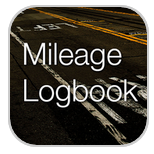
\includegraphics[width=0.48\textwidth]{bilder/mileage}
  \end{center}
\end{wrapfigure}
\textbf{Costs} \euro 3,95 monthly (30 days testversion)
\newline\newline
\textbf{Supported Platforms} Android, \gls{ios}, Windows
\newline\newline
\textbf{GPS} \gls{gps} connection is necessary.
\newline\newline
\textbf{Business/Private mode} You can split your private tracking from your business tracking.
\newline\newline
\textbf{Hardware} No Hardware. App is only used on smartphones.
\newline\newline
\textbf{Access Forms} Web form, App
\newline\newline
\textbf{Manual/Automatic Tracking} automatic and manual
\newline\newline
\textbf{Internet Connection} No internet connection necessary.
\newline\newline
\textbf{Export} It’s possible to export data to a \gls{pdf}, \gls{xml}, Excel or \gls{csv} File.
\newline\newline
\textbf{Other Features} No other features included.
\newline\newline
\textbf{References:} \cite{Fahrtenbuch_Mileage_Book}
\newpage
\clearpageauthor
\section{Trucker Logbook}
\pageauthor{Helena Adam}
\begin{wrapfigure}{r}{0.5\textwidth}
  \begin{center}
    
\includegraphics[width=0.48\textwidth]{bilder/trucker}
  \end{center}
\end{wrapfigure}
\textbf{Costs} free
\newline\newline
\textbf{Supported Platforms} Android, \gls{ios}
\newline\newline
\textbf{GPS} No information
\newline\newline
\textbf{Business/Private mode} Only business mode.
\newline\newline
\textbf{Hardware} No Hardware. App is only used on smartphones.
\newline\newline
\textbf{Access Forms}Web form, App
\newline\newline
\textbf{Manual/Automatic Tracking} manual
\newline\newline
\textbf{Internet Connection} No information
\newline\newline
\textbf{Export} No information
\newline\newline
\textbf{Other Features} No other features included.
\newline\newline
\textbf{References:} \cite{Trucker_Logbook}
\newpage
\clearpageauthor
\section{Logbuch App}
\pageauthor{Laura Rössl}
\begin{wrapfigure}{r}{0.5\textwidth}
  \begin{center}
    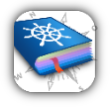
\includegraphics[width=0.48\textwidth]{bilder/logbuchapp}
  \end{center}
\end{wrapfigure}
\textbf{Costs} \euro 5,99 once
\newline\newline
\textbf{Supported Platforms} \gls{ios}
\newline\newline
\textbf{GPS} \gls{gps} connection is necessary.
\newline\newline
\textbf{Business/Private mode} Only private mode.
\newline\newline
\textbf{Hardware} No Hardware. App is only used on smartphones.
\newline\newline
\textbf{Access Forms} App
\newline\newline
\textbf{Manual/Automatic Tracking} No information
\newline\newline
\textbf{Internet Connection} No information
\newline\newline
\textbf{Export} It’s possible to export data to a \gls{pdf} File, Excel or \gls{csv} File.
\newline\newline
\textbf{Other Features} Weather
\newline\newline
\textbf{References:} \cite{Logbuch_App}
\newpage
\clearpageauthor
\section{Drives Fahrtenbuch}
\pageauthor{Paul Zwölfer}
\begin{wrapfigure}{r}{0.5\textwidth}
  \begin{center}
    
\includegraphics[width=0.48\textwidth]{bilder/drives}
  \end{center}
\end{wrapfigure}
\textbf{Costs} Cost free, but there's also a chargeable version where private routes get tracked automatically and you can register more than one vehicle.
\newline\newline
\textbf{Supported Platforms} \gls{ios}
\newline\newline
\textbf{GPS} No information
\newline\newline
\textbf{Business/Private mode} You can split your private tracking from your business tracking.
\newline\newline
\textbf{Hardware} No Hardware. App is only used on smartphones.
\newline\newline
\textbf{Access Forms} App
\newline\newline
\textbf{Manual/Automatic Tracking} The manual tracking version is cost free, but at the chargeable version the automatic tracking is possible and you can split your private and business tracking.
\newline\newline
\textbf{Internet Connection} No information
\newline\newline
\textbf{Export} It’s possible to export data to a \gls{pdf} or \gls{csv} File.
\newline\newline
\textbf{Other Features} 
\begin{itemize}
\item You can use \gls{db} entries as pattern for future tracks
\item Statistics
\item Backups
\item In the chargeable version of the app, you can register more than one vehicle
\end{itemize}
\textbf{References:} \cite{Drives_Fahrtenbuch}
\newpage
\clearpageauthor
\section{Abax Triplog}
\pageauthor{Laura Rössl}
\begin{wrapfigure}{r}{0.5\textwidth}
  \begin{center}
    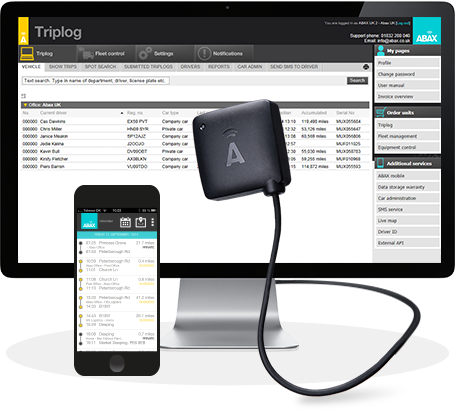
\includegraphics[width=0.48\textwidth]{bilder/abax}
  \end{center}
\end{wrapfigure}
\textbf{Costs} \euro 35,29 monthly \& \euro 249,00 Hardware
\newline\newline
\textbf{Supported Platforms} \gls{ios}
\newline\newline
\textbf{GPS} \gls{gps} connection is necessary.
\newline\newline
\textbf{Business/Private mode} You can split your private tracking from your business tracking.
\newline\newline
\textbf{Hardware}The hardware is very robust and waterproof.
\newline\newline
\textbf{Access Forms}Web form, App
\newline\newline
\textbf{Manual/Automatic Tracking}automatic
\newline\newline
\textbf{Internet Connection}Internet connection necessary.
\newline\newline
\textbf{Export}No information
\newline\newline
\textbf{Other Features} 
\begin{itemize}
\item Contract period of 3 years
\item Lifetime Warranty
\end{itemize}
\textbf{References:} \cite{Abax_Triplog}
\newpage
\clearpageauthor
\section{GPS Log Book}
\pageauthor{Helena Adam}
\begin{wrapfigure}{r}{0.5\textwidth}
  \begin{center}
    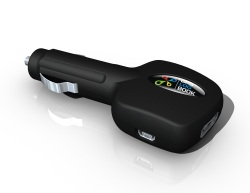
\includegraphics[width=0.48\textwidth]{bilder/GPSlogbook2}
  \end{center}
\end{wrapfigure}
\textbf{Costs} \euro 117,11 + \euro 26,33 per year
\newline\newline
\textbf{Supported Platforms} Web interface
\newline\newline
\textbf{GPS} \gls{gps} connection is necessary.
\newline\newline
\textbf{Business/Private mode} Only private mode.
\newline\newline
\textbf{Hardware}The product consists of a plug in for the car.
\newline\newline
\textbf{Access Forms} Web form
\newline\newline
\textbf{Manual/Automatic Tracking}automatic, manual
\newline\newline
\textbf{Internet Connection}Internet connection is necessary, but data doesn't get transmitted to the \gls{db}.
\newline\newline
\textbf{Export}It's possible to export data to a \gls{pdf} or \gls{csv} File.
\newline\newline
\textbf{Other Features}
\begin{itemize}
\item 5 years data retention 
\item Google Maps integrated
\item 4\gls{mb} log data on the device
\end{itemize}
The GPS Log Book device plugs into a cigarette lighter. You have to copy the data manually from the GPS Log Book on you PC.
\newline\newline
\textbf{References:} \cite{GPS_Log_Book}
\newpage
\clearpageauthor
\section{GPS Log Book Live}
\pageauthor{Helena Adam}
\begin{wrapfigure}{r}{0.5\textwidth}
  \begin{center}
    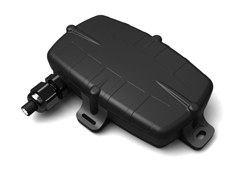
\includegraphics[width=0.48\textwidth]{bilder/GPSlogbooklive!}
  \end{center}
\end{wrapfigure}
\textbf{Costs}\euro 416,69 + \euro 18,16 monthly + Installation \euro 89,87 
\newline\newline
\textbf{Supported Platforms} Web interface
\newline\newline
\textbf{GPS} \gls{gps} connection is necessary.
\newline\newline
\textbf{Business/Private mode}You can split your private tracking from your business tracking.
\newline\newline
\textbf{Hardware}The hardware is very robust and waterproof.
\newline\newline
\textbf{Access Forms}Web form
\newline\newline
\textbf{Manual/Automatic Tracking}automatic + manual
\newline\newline
\textbf{Internet Connection}Internet connection necessary.
Data gets automatically  transmitted to the \gls{db}.
\newline\newline
\textbf{Export}It’s possible to export data to a \gls{pdf} or \gls{csv} File.
\newline\newline
\textbf{Other Features}
\begin{itemize}
\item 5 years data retention  
\item Google Maps integrated
\item Live
\end{itemize}
\textbf{References:} \cite{GPS_Log_Book_LIVE}
\newpage
\clearpageauthor
\section{Gurtam}
\pageauthor{Helena Adam}
\begin{wrapfigure}{r}{0.5\textwidth}
  \begin{center}
    
\includegraphics[width=0.48\textwidth]{bilder/gurtam}
  \end{center}
\end{wrapfigure}
\textbf{Costs} No information 
\newline\newline
\textbf{Supported Platforms} Every platform that supports  Google Chrome 20+, Firefox 15+, Safari 5+, IE 9+, Opera 10+
\newline\newline
\textbf{GPS} \gls{gps} connection is not necessary.
\newline\newline
\textbf{Business/Private mode} You can split your private tracking from your business tracking.
\newline\newline
\textbf{Hardware}No Hardware. App is only used on smartphones.
\newline\newline
\textbf{Access Forms}Web form
\newline\newline
\textbf{Manual/Automatic Tracking}manual
\newline\newline
\textbf{Internet Connection}No internet connection is necessary.
\newline\newline
\textbf{Export}It’s possible to export data to different Files.
\newline\newline
\textbf{Other Features}
\begin{itemize}
\item specifying the beginning and the end of the trip;
choosing type (business/personal trip);
\item specifying initial and final position, duration, mileage data, etc.;
\item manual adding columns containing user notes;
\item logging all the changes;
\item printing or exporting to file;
\item setting Costs per kilometer or per litre (in case of personal trip it helps to calculate the total Costs).
\end{itemize}
\textbf{References:} \cite{Gurtam_Wialon_Driving_Logbook}
\newpage
\clearpageauthor
\section{Maxtech}
\pageauthor{Laura Rössl}
\begin{wrapfigure}{r}{0.5\textwidth}
  \begin{center}
    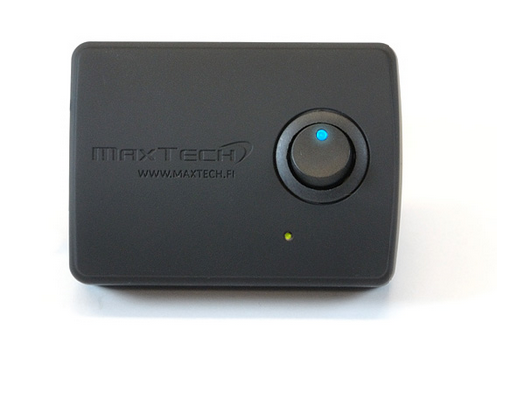
\includegraphics[width=0.48\textwidth]{bilder/logbook}
  \end{center}
\end{wrapfigure}
\textbf{Costs} \euro 189 once
service fee (including the service, SIM card and subscription) is roughly \euro 20 per month (prices excl. VAT)
\newline\newline
\textbf{Supported Platforms} No information given
\newline\newline
\textbf{GPS} \gls{gps} connection is necessary.
\newline\newline
\textbf{Business/Private mode}You can split your private tracking from your business tracking.
\newline\newline
\textbf{Hardware}Hardware is included (picture on the right)
\newline\newline
\textbf{Access Forms}Web form
\newline\newline
\textbf{Manual/Automatic Tracking}automatic and manual
\newline\newline
\textbf{Internet Connection}Yes, data gets transmitted to a server
\newline\newline
\textbf{Export}It is  possible to export data to a \gls{pdf} or \gls{csv} File.
\newline\newline
\textbf{Other Features}
\begin{itemize}
\item An automatic logbook remembers to collect all the drive data so you will no longer forget any travels.
\item data is available anywhere and anytime
\item track your car when the driver is someone else and it also helps if your car is stolen – a tracking device will send the location of your car when it moves.
\item if no internet is available, the drive data gets stored on an internal buffer memory, that can save up to 2000 km
\end{itemize}
Vehicle tracking devices can be installed in three different ways:
\begin{itemize}
\item Cigarette lighter plug
\item OBD connector
\item Fixed mounting to car battery (10V-30V)
\end{itemize}
\textbf{References:} \cite{Maxtech}
\newpage
\clearpageauthor
\section{Tractive}
\pageauthor{Helena Adam}
\begin{wrapfigure}{r}{0.5\textwidth}
  \begin{center}
    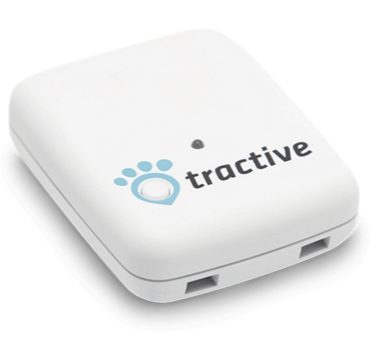
\includegraphics[width=0.48\textwidth]{bilder/tractive}
  \end{center}
\end{wrapfigure}
\textbf{Costs}\euro 79.99 once + \euro 4.99 or \euro 7.49 (Premium) per month 
\newline\newline
\textbf{Supported Platforms} Android and \gls{ios} 
\newline\newline
\textbf{GPS} \gls{gps} connection is necessary.
\newline\newline
\textbf{Business/Private mode} -
\newline\newline
\textbf{Hardware}Hardware is included (picture on the right)
\newline\newline
\textbf{Access Forms} App
\newline\newline
\textbf{Manual/Automatic Tracking} automatic
\newline\newline
\textbf{Internet Connection} Yes, data gets transmitted on the smartphone of the user.
\newline\newline
\textbf{Export}-
\newline\newline
\textbf{Other Features}
\begin{itemize}
\item Sensors for:
\begin{itemize}
\item Movement
\item Speed-Up
\item Temperature
\item Brightness
\end{itemize}
\item Waterproof
\item Alarm, if the pet leaves a certain area
\end{itemize}
\textbf{References:}\cite{Tractive}
\clearpageauthor
\newpage

\section{Summary}
\pageauthor{Helena Adam}
Most of the products only run on very few or only on one platform. There are different versions of software (pay/free)  that divide the user experience in either good or bad way. Our idea is a single software with an extra hardware, web form and a mobile application. This mobile application runs on \gls{ios}, Android and also on Windows phones. These main functionalities should distinguish us from the rest of the market. 

In the analysis above you can see some of the most important competitor products. In our opinion, the largest competitors are Mileage Book and Fahrtenbuch (von Stefan Meyer). These products have many features and a very low or rather no price. However, their product only includes a mobile application.

On the hardware side, GPS Log Book Live and the company maxtech with their product Automatic Driver’s Logbook are our biggest competitors. Although their product is highly innovative, there is no mobile application included. 

Another competitor product is the product of the company Tractive. It has functions like helping you not to lose your pet, tracking its activity and analyzing this data throughout the day.

In conclusion, there are hardly any products consisting of a hardware and a mobile application. We only found two competitors who include both. On the one hand it is Tractive that's original intention is to track your own pets. On the other hand it is Abax Triplog. But this product only runs on \gls{ios} so we are at an advantage. So as you can see, our offer of an hardware and a mobile application that goes with it will distinguish our product from the competitors.
\newline\newline

\begin{tabular}{p{3cm}p{5cm}p{3cm}p{2cm}}
\toprule

  \textbf{Name of \newline Product} & \textbf{Costs} & \textbf{Supported Plattform} & \textbf{includes Hardware} \\
\midrule
  Miles                      & \euro 39,99                                                                                                 & IOS 8                 & No  \\ 
OsmAnd                     & \euro 6,99                                                                                                  & IOS, Tablets, Linux   & No  \\ 
TOMTOM                     & \euro 69,41                                                                                                 & Android and IOS       & No  \\ 
Fahrtenbuch (Stefan Meyer) & \euro 5,99                                                                                                  & IOS                   & No  \\ 
TOUR                       & free                                                                                                        & IOS                   & No  \\ 
Mileage Logbook            & free                                                                                                        & Android               & No  \\ 
Fahrtenbuch (myLogbook)    & \euro 4,98                                                                                                  & Android               & No  \\ 
MyLog GPS Fahrtenbuch      & free                                                                                                        & Android               & No  \\ 
Carpanion                  & free                                                                                                        & Android, IOS, Windows & No  \\ 
Fahrtenbuch Mileage Book   & \euro 3,95 per Month                                                                                        & Android, IOS, Windows & No  \\ 
Trucker Logbook            & free                                                                                                        & Android, IOS          & No  \\ 
Logbuch App                & \euro 5,99                                                                                                  & IOS                   & No  \\ 
Drivers Fahrtenbuch        & free                                                                                                        & IOS                   & No  \\ 
Abax Triplog               & \euro 35,29 per Month + \euro 249 Hardware                                                                  & IOS                   & Yes \\ 
GPS Log Book               & \euro 117,11 + \euro 26,33 per Year                                                                         & Web interface         & Yes \\ 
GPS Log Book Live          & \euro 416,69 + \euro 18,16 per Month + \euro 89,87\\   Installation & Web interface         & Yes \\
Gurtam                     & No information                                                                                              & Web interface         & No  \\ 
Maxtech                    & \euro 189                                                                                                   & No information        & Yes \\ 
Tractive                   & \euro 79,99 once + \euro 4,99 or \euro 7,99 (Premium)per Month                                              & Andoid, IOS           & Yes \\ 
\bottomrule
\end{tabular}
\end{singlespace} 
\clearpageauthor

\setcounter{chapter}{0}
\chapter{Prototype}
\section{Hardware}
\newpage
\section{Software Description}
The software of our \gls{rpi2} consists of two threads and a blocking FileObjectQueue. We get the GPS data from the API and upload it via REST in the Database. 
\subsection{Functions}
First of all a logging property file and a gps property file are loaded. The logging property file contains logging information like the saving location and the maximum number of logging files. The gps property file contains the raspberry id, the server URL and the gps module IP.
\subsection{GPS API}
The API (Gpsd4java) manages the connection with the GPS daemon, which covers receiving data, parsing this information into an useful format and supplying it to the “API Thread”. The GPS data we use consists of the timestamp, coordinateX, coordinateXError, coordinateY, coordinateYError, acceleration, altitude and altitudeError.
\subsection{Tape API}
We implemented this API, because of the problem with saving data into an offline file. This API provides us a FileObjectQueue where we can put and remove our points and this FileObjectQueue is automatically saved in a file. 
\subsection{Save Thread}
The Save thread reads point data from the FileObjectQueue and sends the data to the REST server. When the tracks are written in the database, the Save Thread removes these points from the FileObjectQueue.
\subsection{API Thread}
When the GPS API measures GPS data, the API Thread gets it from the API. The API Thread adds the information about the track and loads it into the FileObjectQueue.
\begin{center}
\includegraphics[width=1\textwidth]{SoftwareDiagram1}
\end{center} 
\subsection{PHP (REST)}
This part of our software is responsible for the upload into the database. The REST server gets the data formatted as JSON.
\begin{center}
\includegraphics[width=1\textwidth]{SoftwareDiagram2}
\end{center} 
\section{Code Structure}
\subsection{Classes}
\subsubsection{GPS.java}
\paragraph{Constructor}
In the GPS.java class, the gpsModuleAddress variable is initialized and gets it is value from the GPSConfiguration.java class.
\paragraph{startGpsdClient}
In the startGpsdClient method, the GPS API is initialized and the validate method from the BL.java class is called every time we get data from the GPS API.
\subsubsection{BL.java}
\paragraph{Constructor}
In this class the FileObjectQueue is created and initialized by the save.jPoint file and the GsonConverter.java class. 
Then a new track is created and at last the SaveDataThread object is initialized and started.
\paragraph{Validate}
Checks if the data from the GPS API is a Number if not it will be set to 0 except the latitude and the longitude. If they are NaN it will do nothing. 
Then it adds the data from the GPS API to the FileObjectQueue.
\paragraph{ProcessData}
This method peeks max 50 and min 15 points from the FileObjectQueue and puts them into a JContainer. Then it sends these points to the DataManager.java class to upload them via the uploadContainer method.
\subsubsection{SaveDataThread.java}
This is an intern Class in the BL class which extends Thread.
\paragraph{Run}
This override method calls the ProcessData method and then waits 1 second.
\subsubsection{Data Manager.java}
\paragraph{Constructor}
Gets the server URL and puts it on the urlString variable.
\paragraph{UploadContainer}
Uploads the JContainer it got, to the Server via Rest 
\subsubsection{JContainer.java}
This is a beans class that contains attributes, getter and setter methods for the respective attribute and a toString method of the JContainer.
\subsubsection{JPoint.java}
This is a beans class that contains attributes, getter and setter methods for the respective attribute and a toString method of the JPoint.
\subsubsection{GPSConfiguration.java}
At the beginning this class loads the logging properties.
\paragraph{InitConfiguration}
Reads the properties for the program from a file and sets these values on the specified variables. If a value is not in the file, it sets a default value. And at the end it closes the file.
\subsubsection{GsonConverter.java}
This class is a converter class that has implemented a FileObjectQueue Converter. In the method from, the bytes from the file are converted, so that they can be saved on the FileObjectQueue. In the toStream method, it is the other way round, so the FileObjectQueue is saved on a file.
\subsection{Class Diagram}
\begin{center}
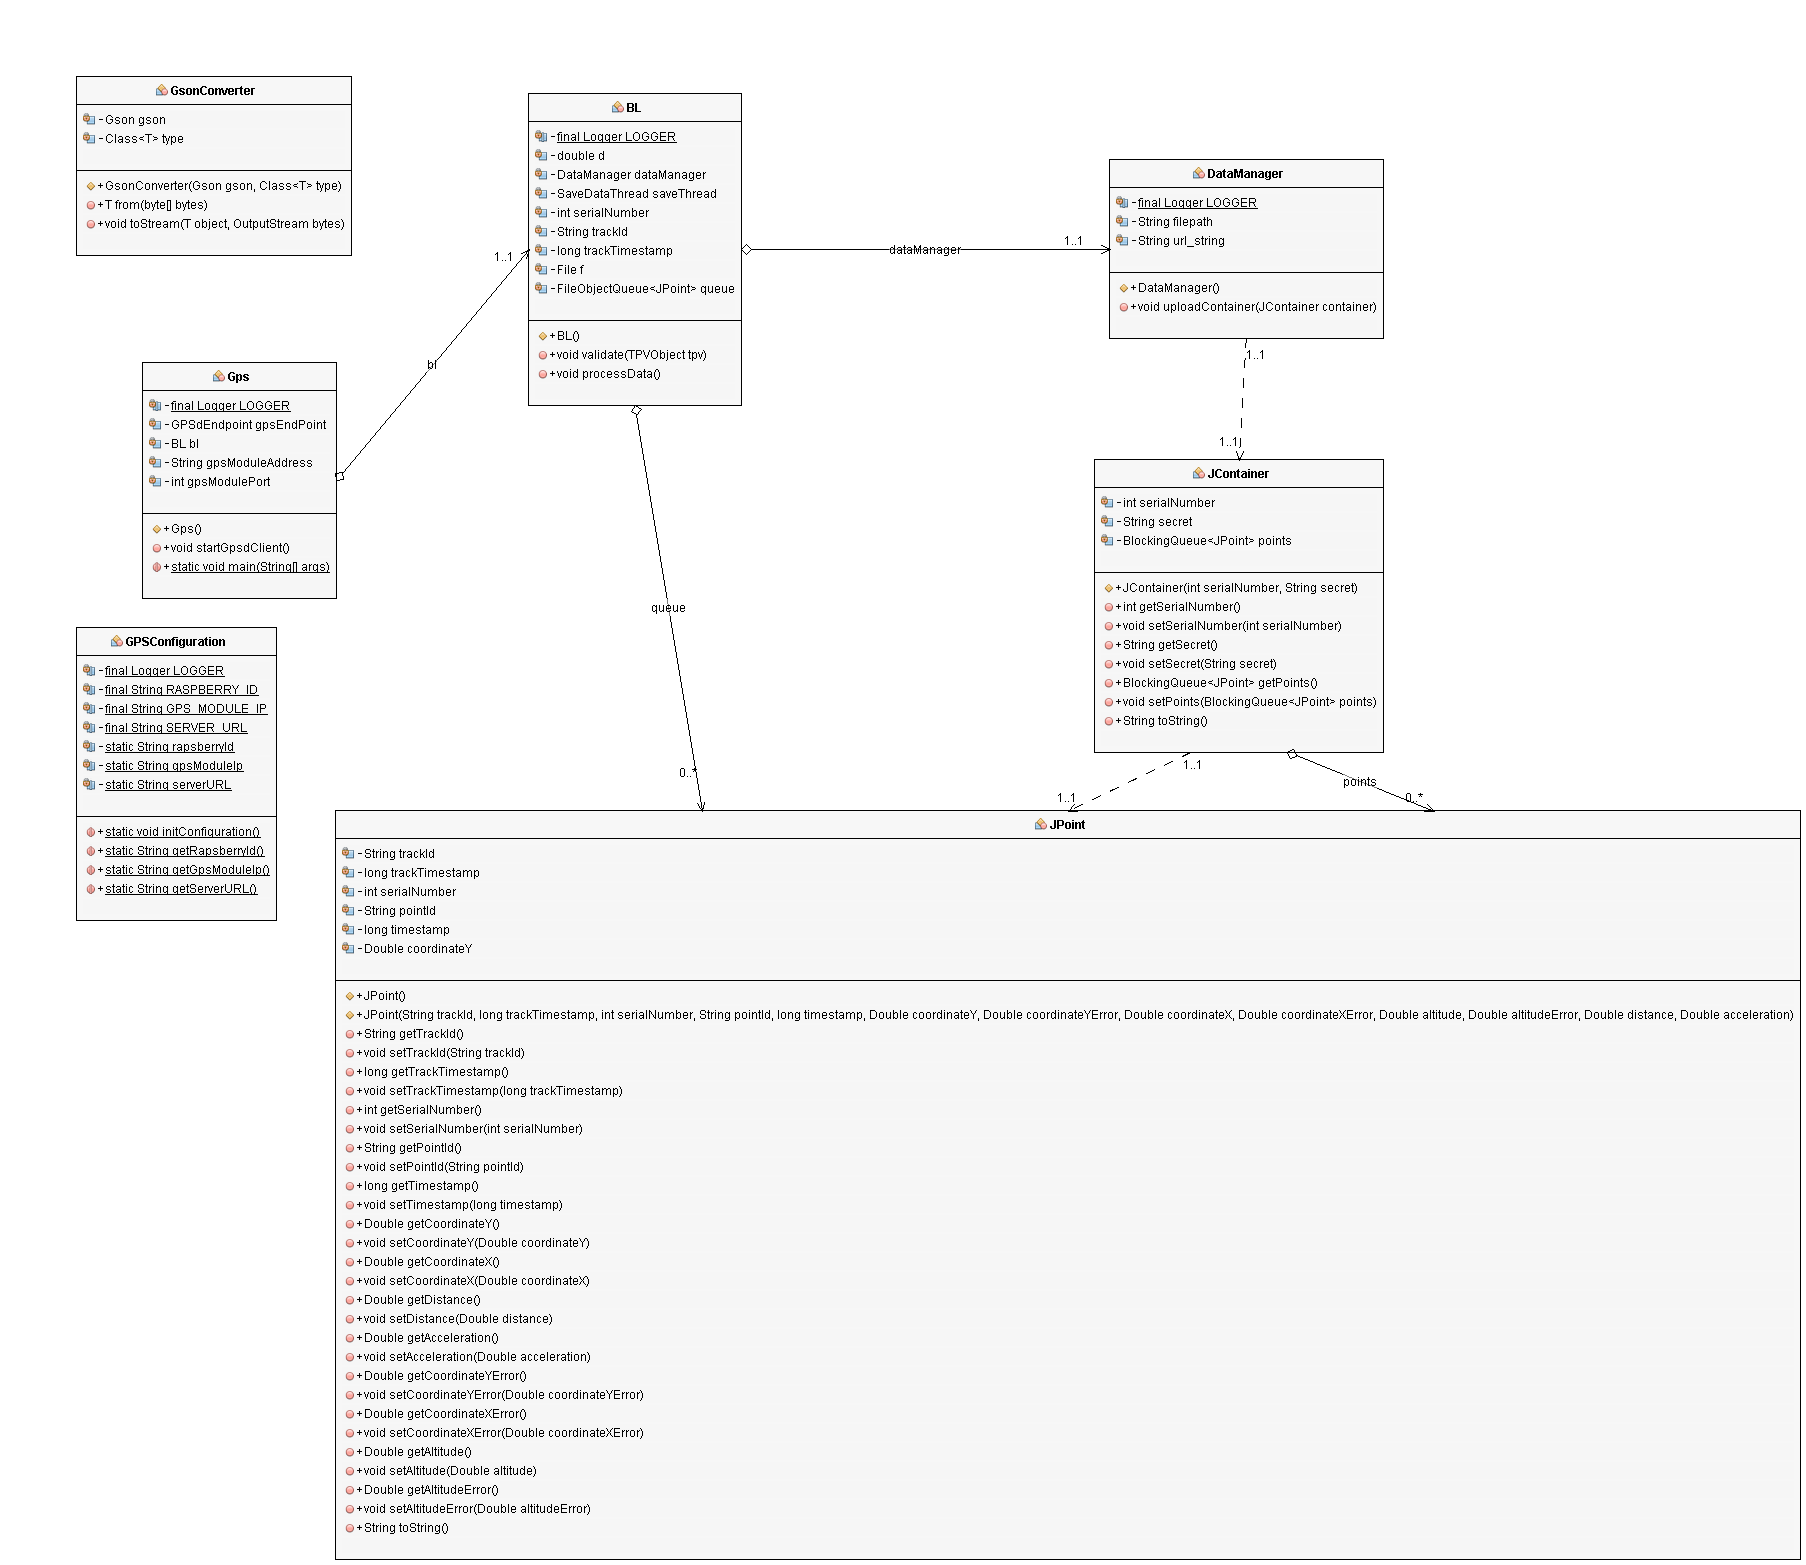
\includegraphics[width=1\textwidth]{GPS_REST_UML_Diagram}
\end{center}
\section{Problems}
\subsection{Uploading into Database}
When we started with this project, we uploaded tracked data directly into the database over a standard java database connection. During our work on this project, we learned the technology hibernate in school so we reconstructed our program and used hibernate. Later our employer told us, that we should use REST to upload data for a higher security level and fewer connections to the database and therefore less overhead. We wrote the REST php script on our own. 
\subsection{Offline Saving}
When the engine stopped while saving data offline, we had a loss of points, because the whole save file we used was overwritten. So we created a copy of this file, removed the data which was already in the database and deleted the original file. Then we renamed the copy to the original file name. Nevertheless, there was still a problem. On the one hand, it was possible that no data was lost, but on the other hand everything could be lost if the power was cut off between deleting the original file and renaming the copy. This is the reason why we use Tape API now. 
\section{Functional Testing}
To ensure functionality of the hardware prototype and the software, we had to do several tests. They reach from logical problems to practical testing on the road.
\subsection{Database Connection Error}
While developing our software, the error handling when loosing database connection was a very important issue. We had to think about different solutions for different code structure because we changed the database connection type. 
\newline \newline
We decided on the connection type which is called REST. When using the connection which relies on a working connection, there had to be a backup plan if exactly this connection is not working anymore.
\newline \newline
In which cases does an connection error occur:
\begin{itemize}
\item internet not working
\item database not working/running
\end{itemize}

We decided on saving points, which cannot be uploaded, into a JSON (save.jPoint). This solution proved to be the most fitting idea we thought of. It perfectly handled the described problems, reliably managed points and the saving mechanism worked phenomenal.
\newline \newline
The same concept is used when the database is offline or not working properly. 

\subsection{Inaccuracy of the GPS Coordinates}
After the first tests, where we tried to get GPS signal, we noticed the inaccuracy of the signal. This inaccuracy gets influenced by several factors. Therefore we had to find out how precise our GPS coordinates are and how much of an imprecision (part of the GPS data we get from our module) there is. 
\newline \newline
We evaluated driven tracks and measured how much distance there is between the actual location and the GPS coordinates received. This difference was about 5 metres, so no problem at all. 
\newline \newline
Due to the fact that we receive how much of an inaccuracy there is in the GPS data, our partner company can easily extract this information and compensate it in the visualization process. To do that even better, we also saved the deviation and the altitude.

\begin{center}
%grafiken der gefahrenen strecken --> claudio
%\includegraphics[width=1\textwidth]{}
\end{center}

\subsection{No GPS Signal}
When handling the GPS inaccuracy, we had to take into account that there could be no signal at all. Therefore we had to decide on a solution when receiving this data and how to handle and save it.
\newline \newline
We tried different solutions, but finally decided on not saving them. It is the most efficient way concerning storage, both offline and online.
\newline \newline
What does not saving data when having no signal mean for us:
\begin{itemize}
\item when there is no GPS signal, there is often also no internet connection
\item which leads to offline stored “null” points
	\begin{itemize}
	\item not saving these null points is the best solution
	\end{itemize}		
\item data extraction for our partner company when displaying the data on maps will be easier
\end{itemize}
\chapter{Database}
One of our four main parts of our diploma thesis was the data design and \gls{db}. We started with creating an entity relationship diagram. This \gls{erd} was the base of our \gls{db}. Because of constant changes in our program structure, we had to change the \gls{db} structure too. 
\section{Entity Relationship Diagram}
\begin{center}
\includegraphics[width=1\textwidth]{ERD_new}
\end{center} 
Customer(svnr, firstname, lastname, dateofbirth, addressIDFK)\newline
Vehicle(vehicleID, svnrFK)\newline
Address(addressID, street, zipcode)\newline
TrackingHardware(serialNumber, svnrFK, description, licenceIDFK)\newline
Licence(licenceID, svnrFK, dateofactivation)\newline
Track(id, serialNumberFK, timestamp)\newline
Point(id, timestamp, (track\_id,track\_serialNumber)FK ,coordinateX, coordinateXError, coordinateY, coordinateYError, acceleration, altitude, altitudeError, distance)\newline
Vehicle\_TrackingHardware(serialNumberFK, vehicleIDFK)
\section{Entities}
\subsection{Customer}
The entity Customer has the social security number as the primary key. Additional attributes are the firstname, the lastname and the date of birth of the person the account belongs to. As you can see in the \gls{erd}, every customer has one reported address and an address can belong to zero or more customers. Due to this, the entity customer contains a foreign key with the id from the address. A customer can only register once, so every customer can have zero or one AdministrationAccount, depending on if he is already registered. Clearly, an account can only belong to one customer so it is well defined who is the owner of the device. There can be a customer who drives more than one vehicle so if he changes to another car, of course he does not have to buy a new device. He can use it for zero or more vehicles. The vehicle is only reported for one customer. This is because if the car is used by more than one person they will not have more than one account. Even if a customer usually only needs one device, it is possible for him to buy zero or more devices. And clearly he does not have to create a new administration account for each of them. But the other way around, every tracking hardware belongs to only one customer.
\subsection{Vehicle}
Every Vehicle has its own unique vehicle id to identify it. This id is also used in our \gls{db} to identify different vehicles. The vehicle is only reported for one customer. This is because if the car is used by more than one person they will not have more than one account. In one vehicle you can place zero or more tracking hardwares and one tracking hardware can be used in zero or more vehicles too, so this is called a “n to m relationship”. We splitted this relationship to an extra entity called Vehicle\_TrackingHardware. This entity contains the two primary keys of the first two tables as primary and foreign key at once.
\subsection{Address}
The entity Address has the unique address id for primary key to identify. It also contains the street name and the zipcode of each address. As you can see in the diagram, one address can belong to zero or more customers but one customer can only be reported to one address.
\subsection{TrackingHardware}
In our \gls{db}, every TrackingHardware is identified by its unique serial number. An additional attribute in this table is the description of the device. One hardware can only belong to one customer and one customer can own zero or more tracking hardwares. So we had to create a foreign key called svnr of the social security number of the Customer. Because of the already mentioned “n to m relationship” between TrackingHardware and Vehicle, you can see an extra entity called Vehicle\_TrackingHardware. With every purchase on a tracking hardware, you acquire an associated Licence. So this table includes the primary key of the Licence called licenceID as a foreign key. A Licence can belong to zero or one device. If the \gls{rpi2} is not purchased yet, the licence is not used. One TrackingHardware has already tracked zero or more Tracks and one Track always belongs to exactly one device.
\subsection{Licence}
The table Licence consists of its own unique licenceID. The svnr is the connection to the Customer Table and is a foreign key in this table. The Licence belongs to one Customer and the Customer can have zero and more Licences. The dateofactivation attribute is, as the names says, the date when the licence was activated on the web portal with the associated device.
\subsection{Track}
Every Track belongs to one TrackingHardware. This Track contains all the Points which belong to this Track. The identifier for the Track is a \gls{uuid}, generated by the program on the \gls{rpi2} and the serialNumber from the TrackingHardware. The table also has a timestamp generated at the start of the program on the \gls{rpi2}.
\subsection{Point}
The greatest part of the information is stored in the Point table. There the identifier is also a \gls{uuid}, generated by the program on the \gls{rpi2}. The primary key is compound of the id, and the primary key from the Track table which is also the foreign key in the Point Table. The identifier from Track is composed of the tack\_id and the serialNumber. The other attributes are the coordinates, the variance of the coordinates, the acceleration, the altitude and the variance of the altitude. The last thing is the distance, which is empty at the time being. Every Point belongs to one Track and every Track contains zero or more points.
\section{\gls{ddl}}
\begin{minted}{SQL}
CREATE TABLE Address(
addressID INT(6) AUTO_INCREMENT PRIMARY KEY,
street VARCHAR(30),
zipcode INT(6)
);
CREATE TABLE Customer(
svnr INT(6) PRIMARY KEY,
firstname VARCHAR(30) NOT NULL,
lastname VARCHAR(30) NOT NULL,
email VARCHAR(50) NOT NULL,
dateofbirth DATE NOT NULL,
addressID INT(6),
FOREIGN KEY fk_Customer(addressID)
REFERENCES Address(addressID)
);

CREATE TABLE Vehicle(
vehicleID INT(8) AUTO_INCREMENT PRIMARY KEY,
svnr INT(6),
FOREIGN KEY fk_Vehicle(svnr)
REFERENCES Customer(svnr)
);

CREATE TABLE Licence(
licenceID INT(8) AUTO_INCREMENT PRIMARY KEY,
svnr INT(6),
dateofactivation DATE NOT NULL,
FOREIGN KEY fk_account (accountID)
REFERENCES AdministrationAccount(accountID)
);

CREATE TABLE TrackingHardware(
serialNumber INT(8) AUTO_INCREMENT PRIMARY KEY,
svnr INT(6),
description VARCHAR(100),
licenceID INT(8),
FOREIGN KEY fk_trackHardw(svnr)
REFERENCES Customer(svnr),
FOREIGN KEY fk_licence(licenceID)
REFERENCES Licence(licenceID)
);

CREATE TABLE VehicleTrackingHardware(
serialNumber INT(8),
vehicleID INT(8),
timestamp DATE NOT NULL,
PRIMARY KEY (serialNumber, vehicleID),
FOREIGN KEY fk_vth_serialNumber(serialNumber)
REFERENCES TrackingHardware(serialNumber),
FOREIGN KEY fk_vth_vehicleID(vehicleID)
REFERENCES Vehicle(vehicleID)
);

CREATE TABLE Track(
id VARCHAR(255),
serialNumber INT(8),
timestamp BIGINT NOT NULL,
PRIMARY KEY(id, serialNumber),
FOREIGN KEY fk_track_serial(serialNumber)
REFERENCES TrackingHardware(serialNumber)
);

CREATE TABLE Point(
id VARCHAR(255),
timestamp BIGINT NOT NULL,
track_serialNumber INT(8),
track_id VARCHAR(255),
coordinateY DOUBLE NOT NULL,
coordinateYError DOUBLE NOT NULL,
coordinateX DOUBLE NOT NULL,
coordinateXError DOUBLE NOT NULL,
acceleration DOUBLE NOT NULL,
altitude DOUBLE NOT NULL,
altitudeError DOUBLE NOT NULL,
distance DOUBLE,
PRIMARY KEY(id, timestamp, track_serialNumber,track_id),
FOREIGN KEY fk_point_track(track_serialNumber, track_id)
REFERENCES Track(serialNumber, id)
);
\end{minted}
\section{\gls{dml}}
\begin{minted}{SQL}
INSERT INTO Address(addressID, street, zipcode)
VALUES(1,'Blumenweg',8430);
INSERT INTO Customer(svnr, firstname, lastname, email, dateofbirth, addressID)
VALUES(4523, 'Karl', 'Huber', 'karl.huber@gmail.com',
DATE_FORMAT('1970-12-09','%Y-%m-%d'),1);
INSERT INTO Vehicle(vehicleID, svnr)
VALUES(832,4523);
INSERT INTO Licence(licenceID, svnr, dateofactivation)
VALUES(832495,4523,DATE_FORMAT('2016-01-20','%Y-%m-%d'));
INSERT INTO TrackingHardware(serialNumber, description, licenceID)
VALUES(1234, 'Karlis Raspi', 832495);
INSERT INTO VehicleTrackingHardware(serialNumber, vehicleID, timestamp)
VALUES(1234, 832, DATE_FORMAT('2016-01-24','%Y-%m-%d'));
INSERT INTO Track ('id', 'serialNumber', 'timestamp') 
VALUES('018f8ff5-395b-42d2-b2f6-5c976292cd5e', 1234, 1455535245172);
INSERT INTO Point ('id', 'timestamp', 'track_serialNumber', 'track_id', 
'coordinateY', 'coordinateYError', 'coordinateX', 'coordinateXError', 
'acceleration', 'altitude', 'altitudeError', 'distance') 
VALUES('007dae03-c915-4aae-baf9-2b7c42a41e43', 1455535245172, 1234, 
'1f114f58-fd0c-4da6-a1b6-571ae9e79748', 46.78029, 14.815, 15.54794, 10.697, 
0.103, 277.3, 18.17, 0),
('dedc843e-e29b-4a0d-b32d-20cb718088ea', 1455535282394, 1234, 
'1f114f58-fd0c-4da6-a1b6-571ae9e79748', 46.780401667, 14.815, 15.547526667, 
10.697, 7.562, 279, 16.56, 0);
\end{minted}
\section{Problems}
While we tried to insert testing data into our \gls{db}, we noticed that it wasn’t possible to save the timestamp as milliseconds. After researches, we discovered that the problem was the version of our \gls{mysql} \gls{db} (version 5.5.46). Due to this problem we had to change the datatype of our timestamp into bigint.
\chapter{Wireframing}
\pageauthor{Laura Rössl, Paul Zwölfer}
\section{Smartphone}
The design for the smartphone consists of four different pages. 
\subsection{Login}
The login dialogue is the first page you see. There are two input fields; for the username and the password. Below these input fields there is the login button to confirm and login. Then there is a check box to stay logged in.

The link if the password has been forgotten and a button to register and create a new user account are the last things on this page.
\subsection{Menu}
The menu pops up from the left edge as you can see on the picture down below. It can be chosen between viewing the tracks, customize settings, view statistics and logout.
\subsection{Tracks}
On the tracks page a map shows the last track by default but on the bottom any available track can be chosen to view it.
\subsection{Settings}
Under settings, basically changes like edit the mail address or change the password of the account can be applied, but also if the default track type should be private or public.
\subsection{Statistics}
It’s possible to view a graph where information of driven tracks are shown. Every registered car of this account can be chosen to view its graph and additionally, it’s selectable if the displayed data was tracked within the last week, month or year.
\begin{center}
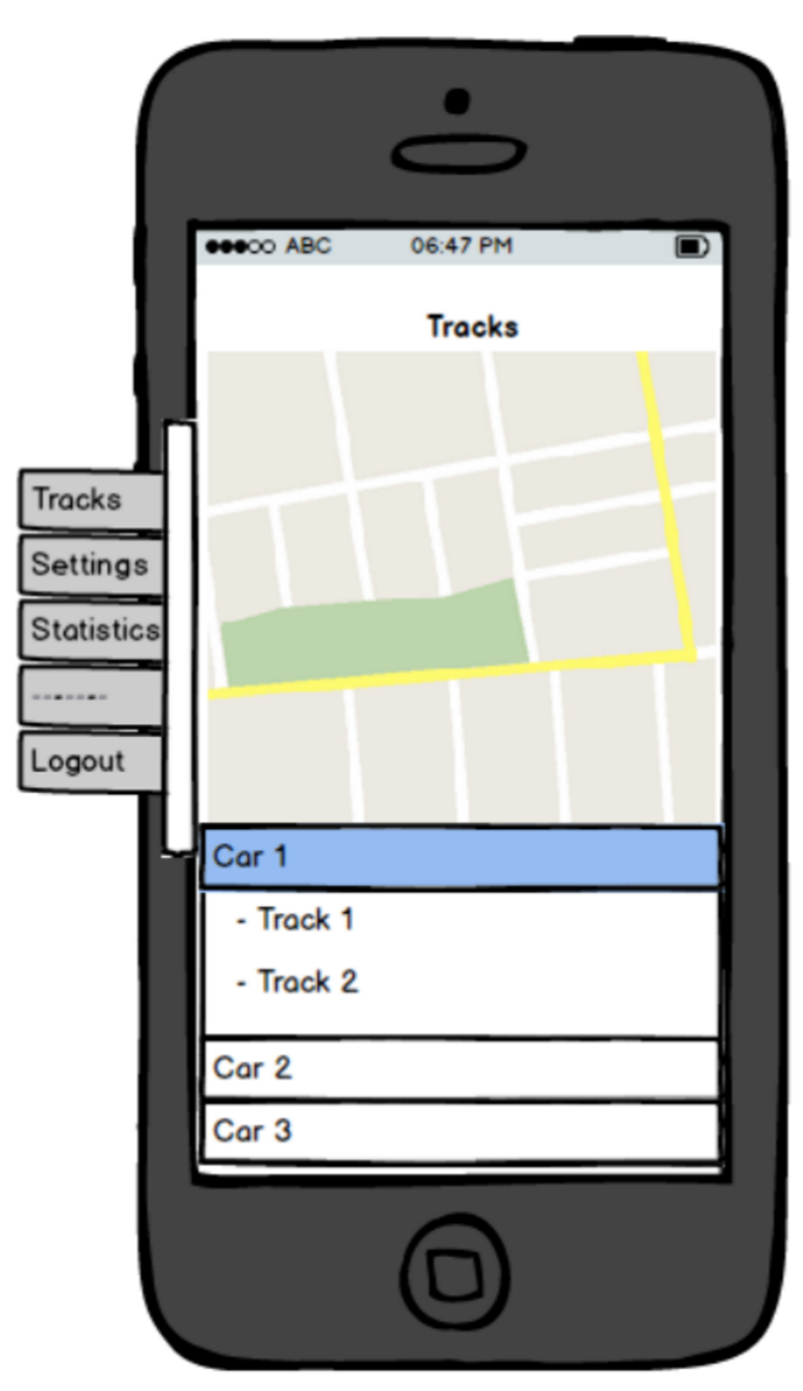
\includegraphics[width=0.4\textwidth]{bilder/Smartphone}
\end{center}
\section{Tablet}
The wireframing we created for the Tablet design is nearly similar to the smartphone design. Except of a few extensions, such as for renaming the device and editing tracks more precisely.
\subsection{Login}
The login dialogue is the first page you see. There are two input fields for the username and the password. Below these input fields there is the login button to confirm. Then there is a check box to stay logged in.
The link if the password has been forgotten and a button to register and create a new user account are the last things on this page.
\subsection{Menu}
The menu pops up from the left edge as you can see on the picture. It can be chosen between viewing the tracks, customizing settings, viewing statistics, renaming the device, registering a car and a logout.
\subsection{Tracks}
On the tracks page a map shows the last track by default. A track can be selected and there is the option to edit or merge a route.
\subsection{Settings}
Under settings, basic changes like editing the mail address or changing the password of the account can be applied, but also if the default track type should be private or public.
\subsection{Renaming Devices}
The \gls{rpi2} gets a random identification name from the start. It is possible edit this name if the user wishes so.
\subsection{Registering Car}
Over the account settings, it is possible to registrate a new car with your licence.
\subsection{Statistics}
It’s possible to view a graph where information of driven tracks is shown. Every registered car of this account can be chosen to view its graph and additionally, it’s selectable if the displayed data was tracked within the last week, month or year.
\begin{center}
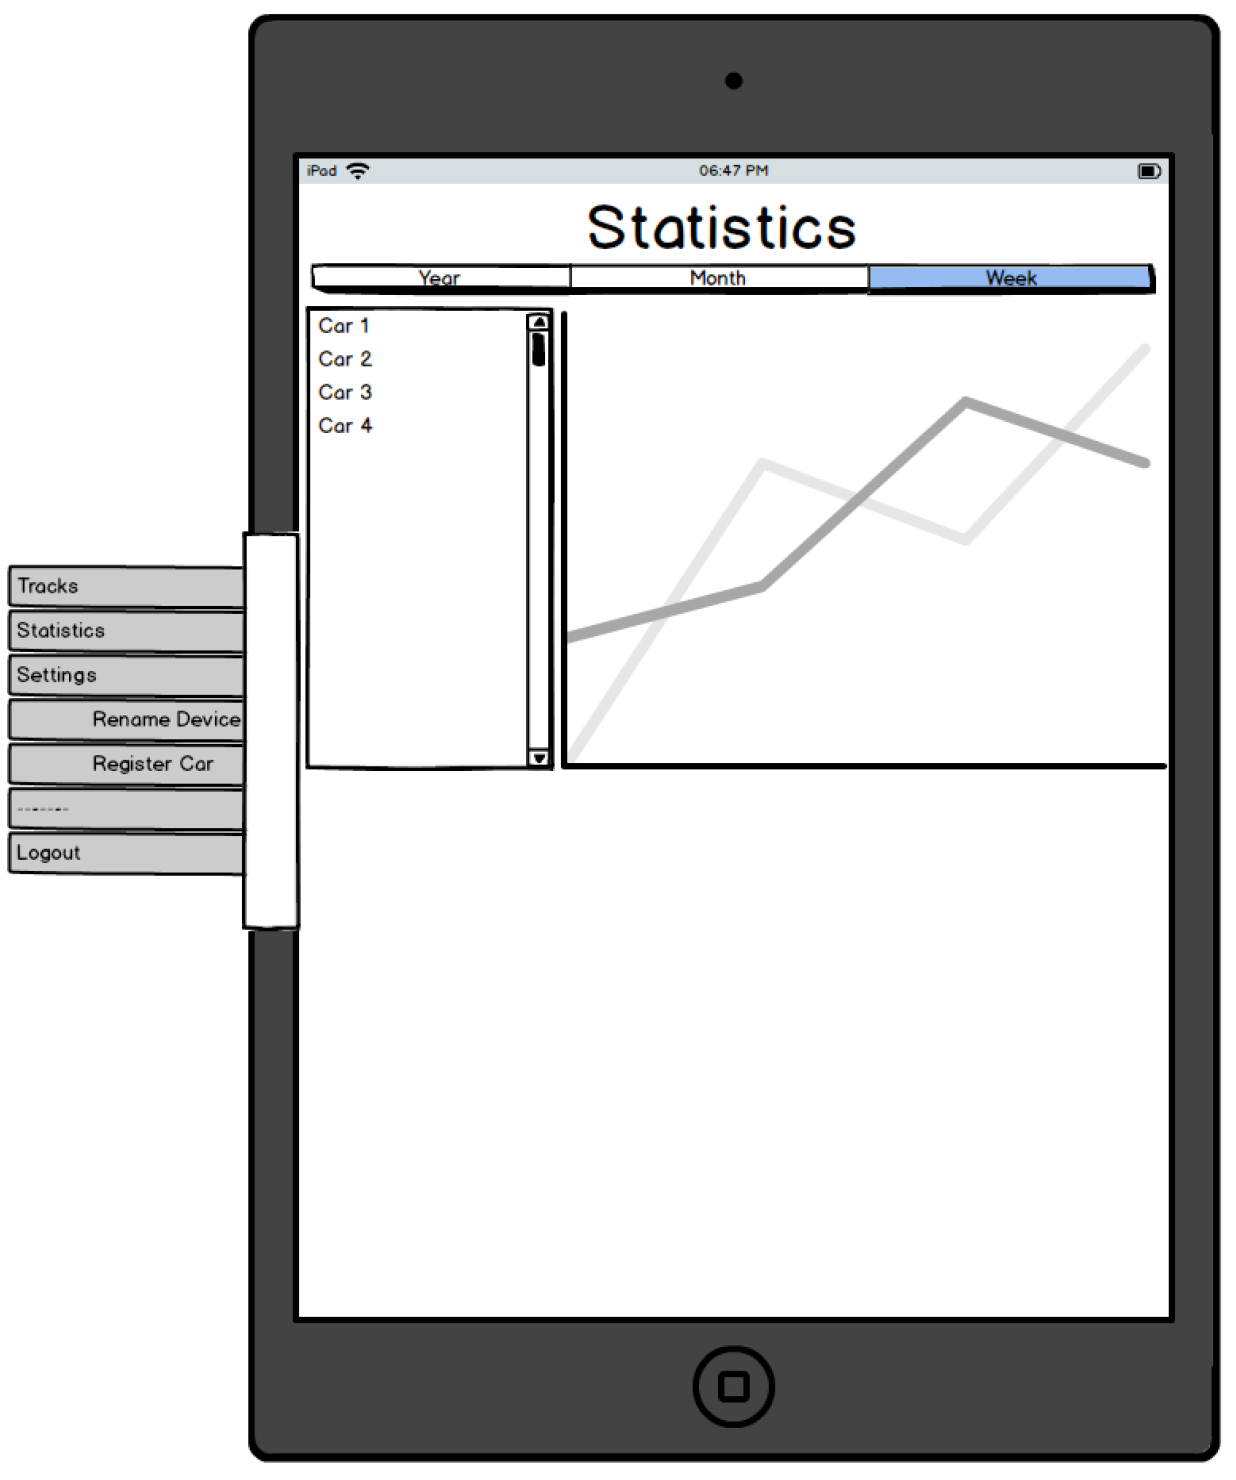
\includegraphics[width=0.625\textwidth]{bilder/Tablet}
\end{center}
\section{Web Portal}
\subsection{Home}
Before the user is logged in, information about the product is shown on this page.

After the login, all tracks are shown and it is possible to change the tracks from private to public.
\subsection{Login}
The login dialogue is the first page you see. There are two input fields for the username and the password. Below these input fields there is the login button to confirm and login. Then there is a check box to stay logged in.
The link if the password has been forgotten and a button to register and create a new user account are the last things on this page.
\subsection{Settings}
Under settings, basic changes like editing the mail address or changing the password of the account can be applied, but also if the default track type should be private or public.
\subsubsection{Registering Car}
Over the account settings, it is possible to registrate a new car with your licence.
\subsubsection{Renaming Device}
The \gls{rpi2} gets a random identification name from the start. It is possible edit this name if the user wishes so.
\subsection{Track}
On the tracks page a map shows the last track by default. It can be chosen between the cars and the tracks of the respective cars can be viewed.
\subsubsection{Edit}
If a track is selected, there is the possibility of editing it. If the route isn’t complete or must be changed in any way, it can be done over the web portal. Should it happen that one track is splitted up into two or more tracks because of complications, you can merge them into one whole route.
\subsubsection{Create}
Here a new track can be created manually over the web portal and the route of the track can be chosen. It’s possible to set the start and end position of the new track and changing the route by pulling the line to the desired way.
\subsection{Statistics}
It’s possible to view a graph where information of driven tracks are shown. Every registered car of this account can be chosen to view its graph and additionally, it’s selectable if the displayed data was tracked within the last week, month or year.
\subsection{Menu}
The menu from the homepage contain home, tracks, statistics, settings and login. The menu item tracks contains subitems called edit and create. The subitems of settings are register car and rename device.

\begin{center}
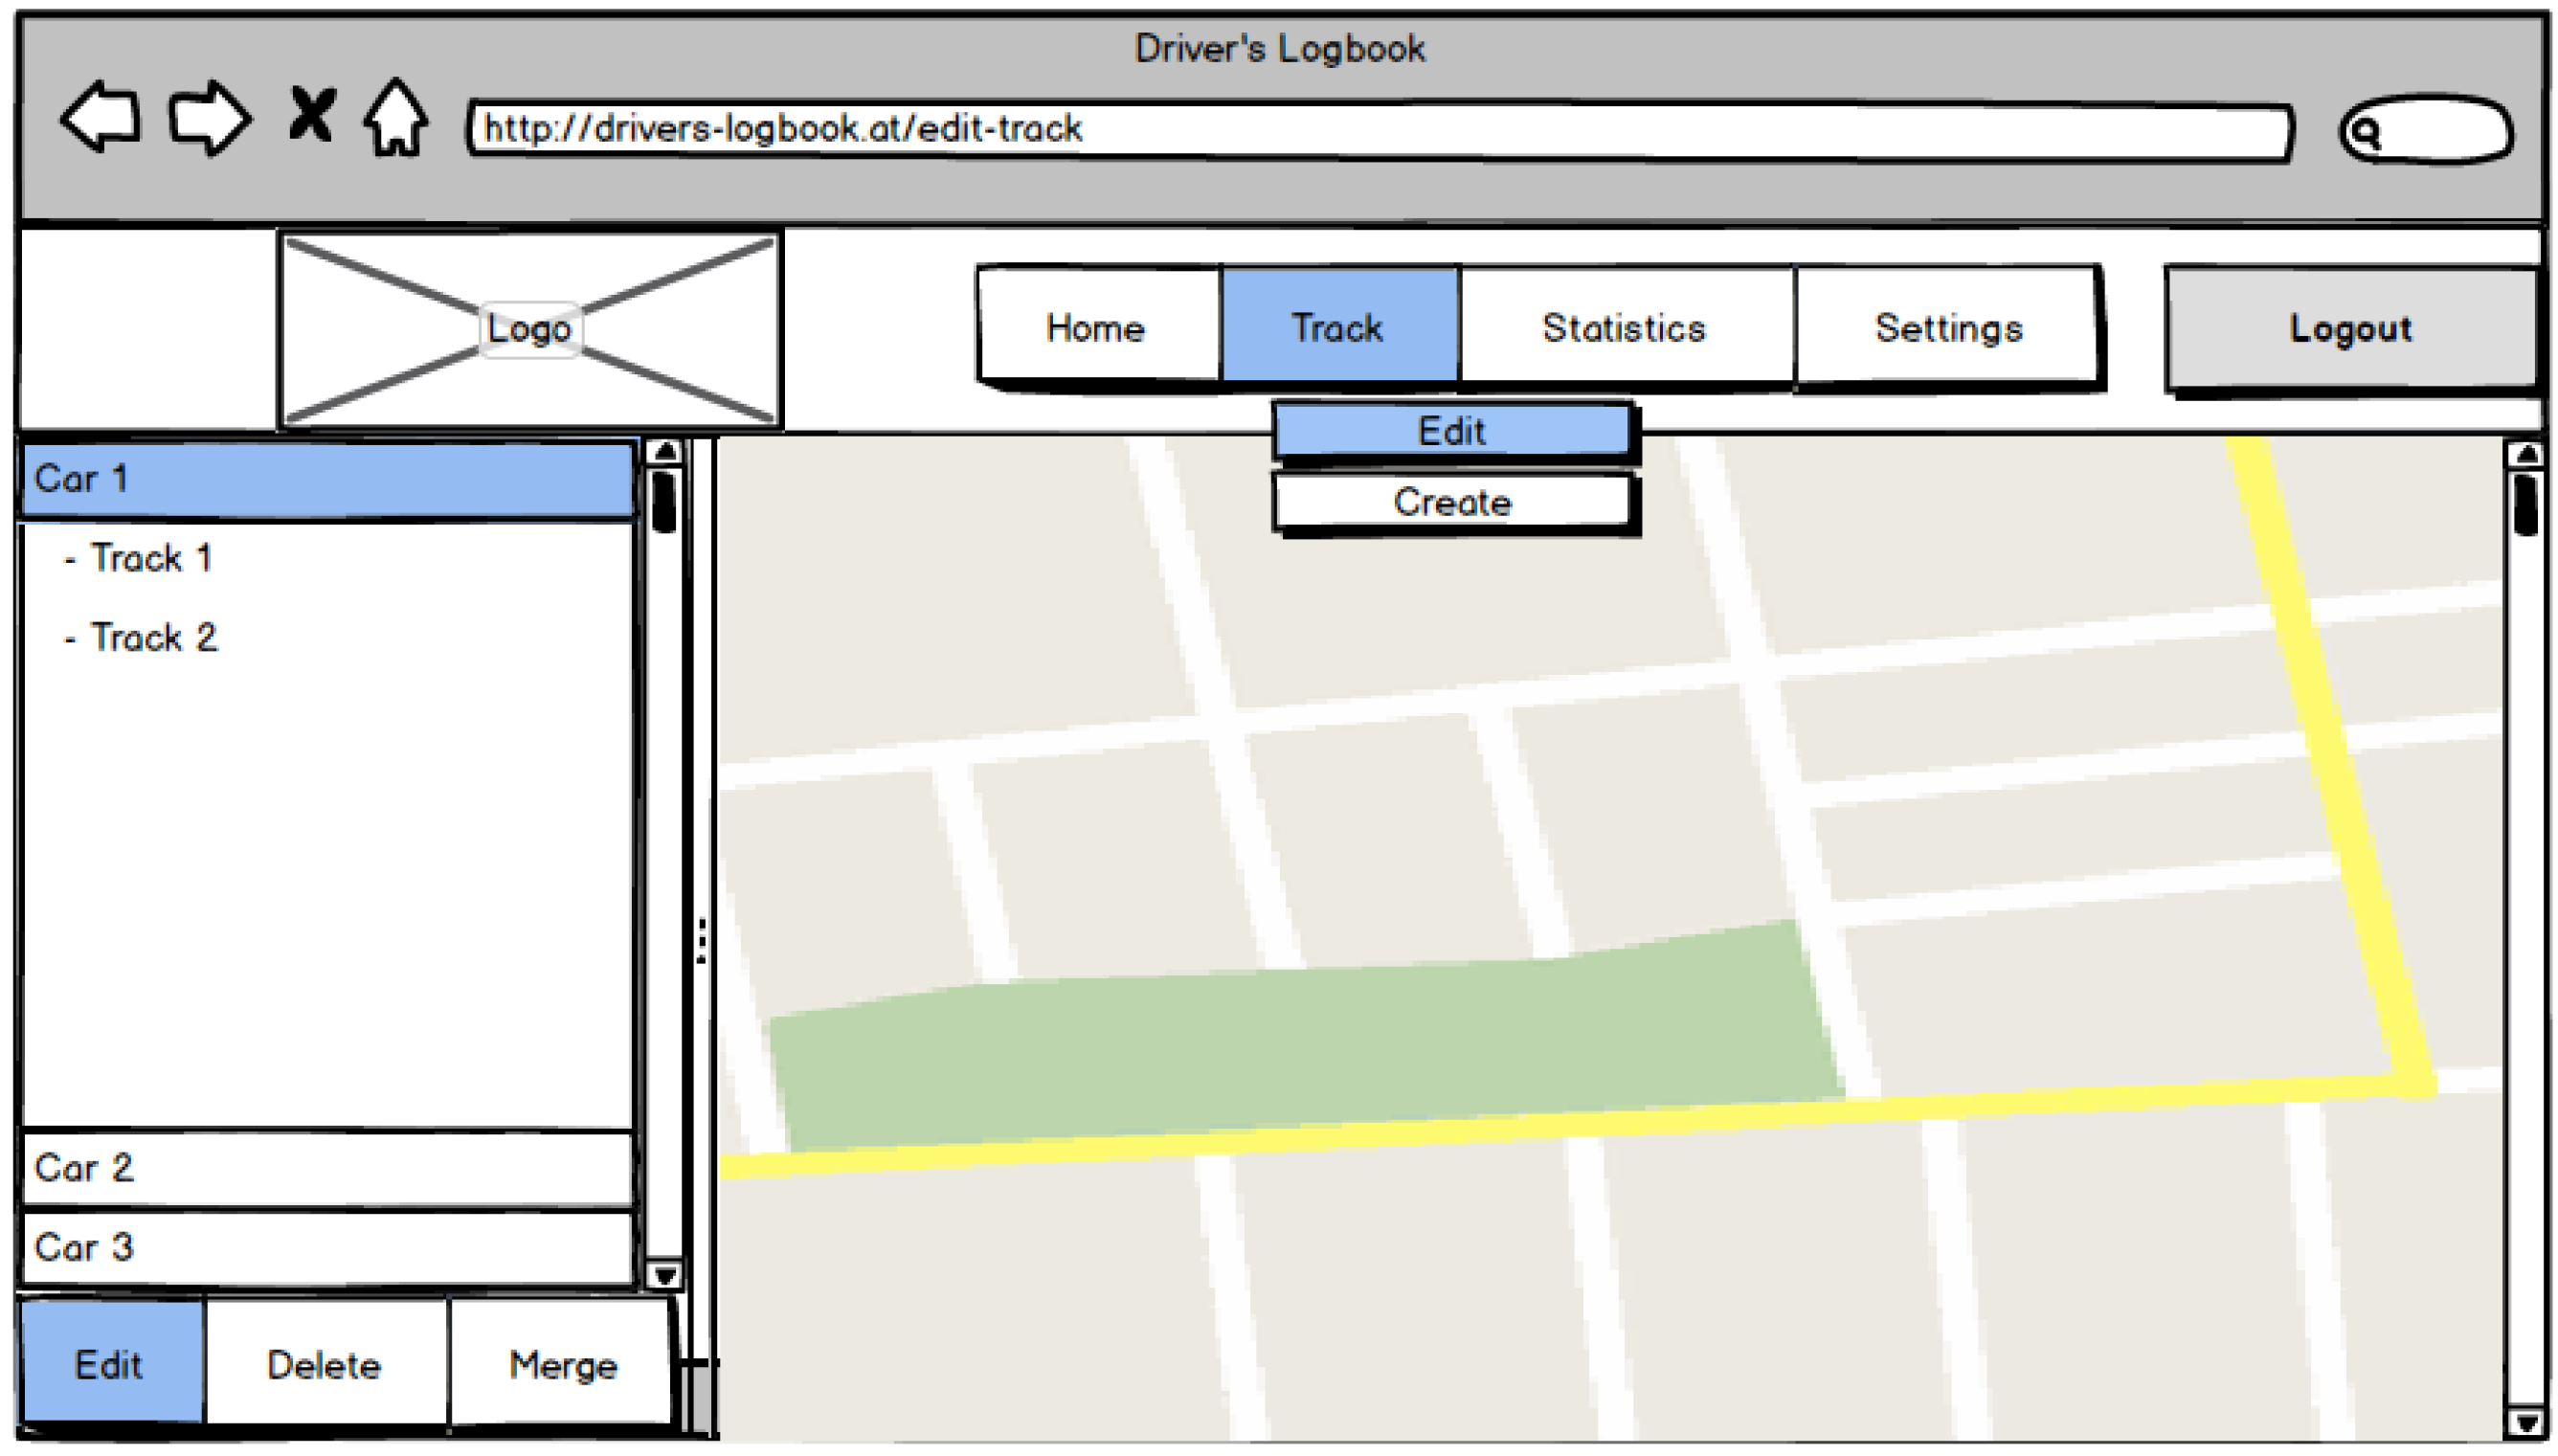
\includegraphics[width=1\textwidth]{bilder/WebPortal}
\end{center}
\clearpageauthor
\chapter{Optional Uses}
The basic concept of our product was to track driven distances of a car you use for private and business purposes. Nevertheless, we thought about other possible uses for this product.
\section{Taxi}
One of our ideas for optional uses was for a taxi company. Our product could be placed in the taxi, the taxi driver presses a button if a new customer enters the car and the device calculates the price of the taxi ride based on the distance, the velocity and the fix basic costs. 
\section{Car Renting}
A car renting company usually gets paid for renting their cars per day. Our product could help them to control the use of their cars. Our product could track the distances the customer took so the company could calculate a suitable price. 
\section{Train Controller}
We thought about the optional use as a train controller for checking the current location of a train, check for complications and preventing delays. It would be also possible planning ahead to avoid incidents and more delays.
\section{Mowing Machine}
There are already mowing machines which drive around in your garden on their own and they are already able to discover the shape of your ground. Using our product, you could extend the conventional device so you can choose between predetermined tracks which your mowing machine could take. It would also be possible to control your mowing machine over a mobile application to change the direction or stop mowing.
\section{Helicopter}
Another optional use for our product could be a controlling device for a helicopter. Choosing a flying track or checking the position and the track of the helicopter could be possible.
\section{Pet Tracking}
Another possibility for our product is to power the device with an battery pack and use it to track your pet. For example if you have a dog or a cat, you can put it on their collar for example and watch where it is and where it goes.
\begin{center}
\includegraphics[width=0.85\textwidth]{bilder/UseCase}
\end{center}

\chapter{User Manual}
\section{General}
First of all, thank you for buying our product. With your purchase on our product, you acquired a licence. Now you can register on our web portal and create your own account. Using your purchased licence, you can activate the product and connect it with your user account. You can also transfer the product with the related licence to another user account. Over the web portal, you can log in and view tracks, visualize them and eventually edit them.
\section{Installation Regulations}
The product has to be placed in the car and connected with the cigarette lighter receptacle to get power. When starting the engine of the vehicle, the device powers itself up and starts searching for a \gls{gps} signal.
\section{LEDs}
When you connect the product to a power source you will see some LEDs light up.
There are three LEDs. A red one on top of the \gls{rpi2}, which is for \gls{gps} module and two on the opposite side of the USB ports which are red and green.
When the red LED next to the green one is on, the \gls{rpi2} gets power.
The green LED on the \gls{rpi2} lights up when the device boots and prepares itself for tracking. When it is ready and it receives data it flickers quick.
And if the red LED on the \gls{rpi2} \gls{gps} module blinks once per second, it has a \gls{gps} signal
\section{Warnings}
\begin{itemize}
\item This product shall only be connected to an external power supply rated at 5V dc, and a minimum current of 500-700mA for model A and 700-1200mA for model B. Any external power supply used with the \gls{rpi2} shall comply with relevant regulations and standards applicable in the country of intended use. 
\item This product should not be overclocked as this may make certain components very hot. 
\item This product should be operated in a well ventilated environment and the case should not be covered. 
\item This product should be placed on a stable, flat, non-conductive surface in use and should not be contacted by conductive items. 
\item The connection of unapproved devices to the GPIO connector may affect compliance or result in damage to the unit and invalidate the warranty. 
\item All peripherals used with the \gls{rpi2} should comply with relevant standards for the country of use and be marked accordingly to ensure that safety and performance requirements are met. These articles include but are not limited to keyboards, monitors, and mice used in conjunction with the \gls{rpi2}.
\item Where peripherals are connected that do not include the cable or connector, the used cable or connector has to offer adequate insulation and operation in order that the requirements of the relevant performance and safety requirements are met.
\end{itemize}
\paragraph{To avoid malfunction or damage to your device please observe following:}
\begin{itemize}
\item Do not expose it to water, moisture or place on a conductive surface whilst in operation.
\item Do not expose it to heat from any source; the \gls{rpi2} is designed for reliable operation at normal ambient room temperatures.
\item Take care whilst handling to avoid mechanical or electrical damage to the printed circuit board and connectors.
\item Avoid handling the printed circuit board while it is powered. Only handle by the edges to minimise the risk of electrostatic discharge damage.
\item The \gls{rpi2} is not designed to be powered from a USB port of the other connected equipment. If this is attempted, it may malfunction.
\end{itemize}




\chapter{Future Work and Ideas}
Due to our limitation in time, we cannot infinitely improve our program. Therefore we sum up our future ideas on what could be implemented or improved. Of course, we only write about the things that came up to our minds, and therefore this is just a small list.
\paragraph{Security between RPi2 and REST service}\mbox{}\\
As we found out during the implementation process, \gls{rest} supports an encryption process. After consulting the partner company, we decided on not using the encryption on the prototype.
\paragraph{Access via SSH over UMTS}\mbox{}\\
It should be possible to access the \gls{rpi2} over the internet via \gls{ssh} for remote maintenance.
\paragraph{Critical error reporting}\mbox{}\\
If a severe problem happens, \gls{rpi2} should be able to report that problem so that it can be fixed.
\paragraph{Mobile Application/Webform}\mbox{}\\
Using the wireframing of the webform and mobile devices, it is possible to create an access interface that can be accessed via a web browser or a mobile application.
\paragraph{Putting the GPS Points on the street}\mbox{}\\
As shown in the Functional Testing part, the \gls{gps} data is rather inaccurate. Therefore our partner company has to interpolate and/or use the inaccuracy we add to the uploaded data. This task was not possible not accomplish in the given time, but could be implemented afterwards.

Compensating the inaccuracy will help to get an exact distance measurement and provide a better user experience.
\paragraph{Optimize Http overhead}\mbox{}\\
If there are many points on the \gls{rpi2}  and the connection is established, the connection should only be closed after sending all the Points.

\chapter{Tools and Technologies}
\section{Java}
We decided on using JAVA, because it runs on every platform, is easy to implement and our partner company could use it on Android devices too. Also the fact that every member of the group got 5 years of programming experience in this language shows that it is the most fitting choice for us.
\section{TAPE API}
We implemented this API, because of the problem with saving data into an offline file. This API provides us a FileObjectQueue where we can put and remove our points. This FileObjectQueue is automatically saved in a file.
\section{GPS API}
This API was rather hard to find because there are few possible ways of handling the GPS data from an RPi2 in JAVA. Nevertheless, we read through the excellent documentation and found ways to use this API in an easy way.
\section{RASPBIAN}
As we tried out different things in linux on the Raspbian Wheezy during our NVSU lessons, it showed its potential. Another point why we used it, was that it was constructed to work perfectly with the RPi2. Therefore, our first choice was this image for our RPi2. Later we found out, that Raspbian Wheezy was not supported any more and so we had to switch to Raspbian Jessie Lite. Raspbian Jessie Lite is only a command line operating system, so it is perfect for our project.
\section{PHP}
The usage of PHP is based on REST. It's functioning kind of like a server, which connects to the database, uploads the GPS data and disconnects.
\section{BalsamiQ}
We used this tool to provide our wireframing plans. It was provided by our employer because they have made a very good experience when using it.
\section{GIT}
When working in a group, a good collaboration tool is needed. Our choice was GIT because we only made negative experiences.\newline
Unfortunately, we had problems at the beginning of our software development. Everytime we tried to "PULL" committed changes, we encountered a merge conflict. This conflict somehow followed us through the whole development phase.\newline
At the end, we also used GIT for LATEX cooperation. Due to the usage of the GIT console, it was a very pleasant experience.
\section{MySQL}
Our employers standard as database technology was MySQL. Due to our experience we got in our DBI lessons, we encountered no problems.
\section{Netbeans}
The programming IDE of our choice was Netbeans. Over 4 years of experience in the same working environment payed off when working on a new, more complex set of problems on our own. These problems reached from logical errors to migrations of completely new programme structures. 
\section{Google Drive}
At the beginning and almost through the whole project, we used Google Drive for document management, time reporting and organization.\newline
The main Google products we have used were Google Docs and Google Tables.\newline
Collaborating was the main reason why we used especially this technologies. It worked trouble-free and had option to restore older versions of documents, which came in handy from time to time.
\section{Notepad++}

\section{LaXeT}

\section{Textmaker}

\section{draw.io}

\section{XAMPP}

\section{phpMyAdmin}

\section{Hangouts}


\printglossaries

\nocite{*}
\newpage
\addcontentsline{toc}{chapter}{Bibliography}
\printbibliography

\end{document}